\documentclass{article}
% Packages
\usepackage{titlesec}
\usepackage{indentfirst}
\usepackage{amsmath, amsthm, amssymb, graphicx}
\usepackage{graphicx}
\usepackage[pages=-]{background}
\usepackage{xcolor}
\usepackage{caption}
\usepackage{booktabs}
\usepackage{hyperref}
\usepackage{bookmark}
\usepackage[left=25mm, right=25mm, bottom=35mm]{geometry}
\usepackage{float}
\usepackage{array}

\backgroundsetup{
  scale=1,
  angle=0,
  opacity=1,
  color=black,
  position=current page.north east,
  vshift=-1.5cm,
  hshift=-2.5cm,
  contents={
    
\includegraphics[width=2cm]{../source/Universitaet_Logo_RGB.pdf}
  }
}
% Title
\title{Satellite Lab1}
\author{Group6: Zhengyang Hua, Xipeng Li, Yushuo Feng}
\date{\today}


\begin{document}

\maketitle
\tableofcontents

\section{Introduction}
This lab focuses on the geometry and kinematics of the polar region. 
And our group use the IGS products(station positions) to estimate the time series, horizontal and vertical velocities of three stations: KIRU, MORP, and REYK, whose locations are shown in the following figure:
In the final part, we compare these result with the plate tectonics model NUVEL 1A and GIA models.
\begin{figure}[htbp]
  \centering
  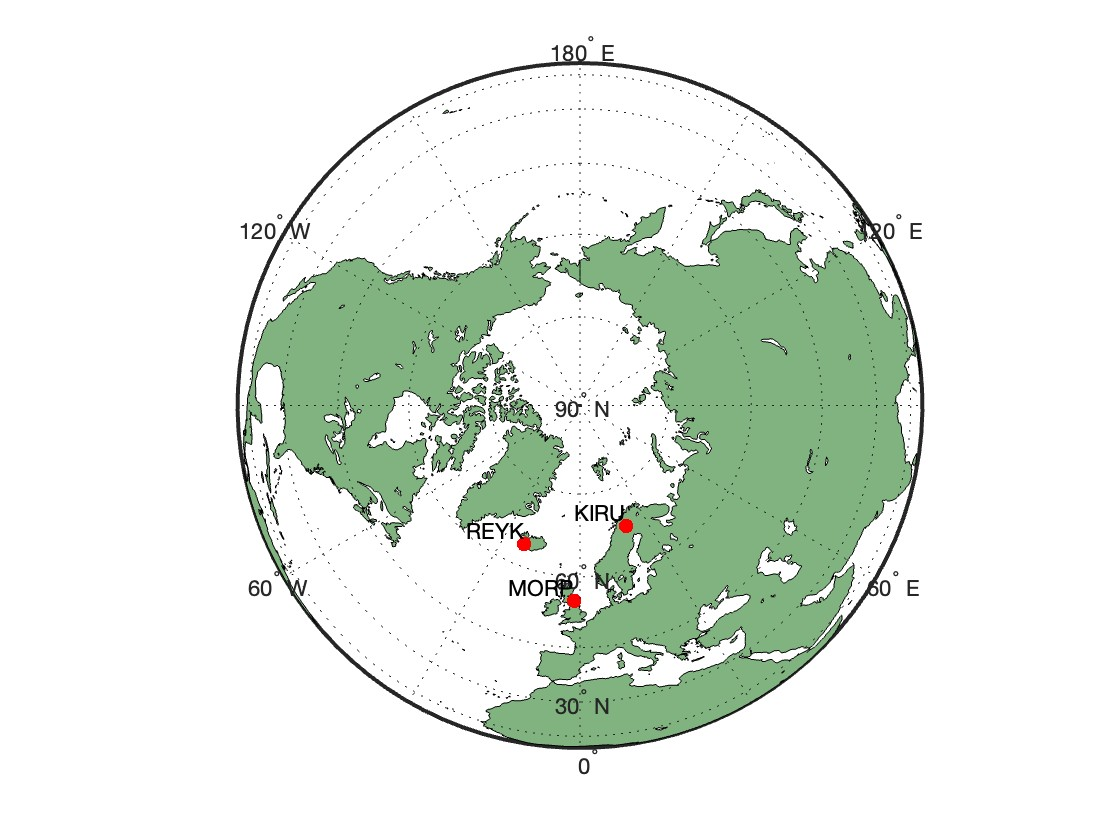
\includegraphics[width=8cm]{../result/point/Point.jpg}
  \captionsetup{skip=0.2cm}
  \caption{Station Positions}
  \label{Intro:station}
\end{figure}

\section{Data Description}
\subsection{ITRF2008 IGS station}
The ITRF is The International Reference Frame,  
and ITRF2008 is a realization of the International Terrestrial Reference System 
that uses as input data time series of station positions and EOPs provided by the Technique Centers of the four space geodetic techniques (GPS, VLBI, SLR, DORIS).

In the file "ITRF2008\_GNSS.SSC.txt", we can find the coordinates of different stations at epoch 2005.0.
 and Time is given as the yyyy.yyyy format, which is the number of decimal years:
\begin{figure}[htbp]
    \centering
    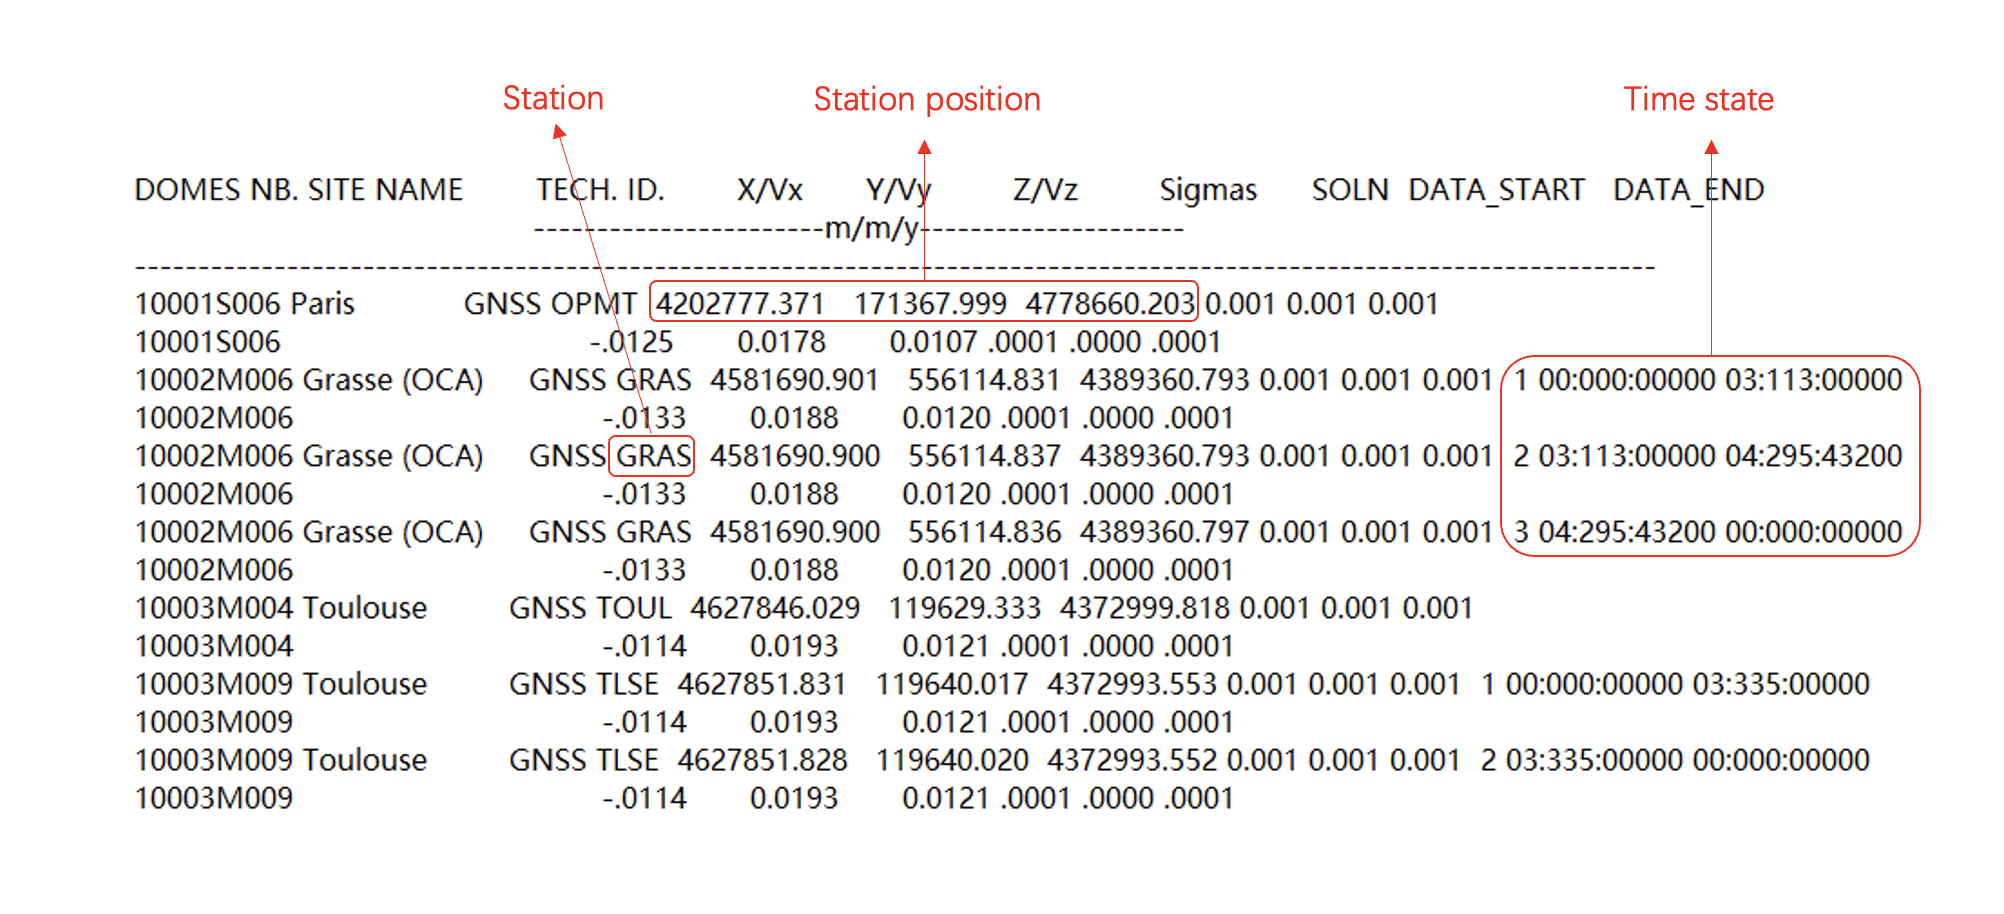
\includegraphics[width=11cm]{./source/ITRF2008.png}
    \caption{ITRF2008\_GNSS.ssc.txt Description}
    \label{fig:ITRF2008}
\end{figure}
\subsection{Station GPS Obversations}
We were responsible for the computation of the positions and movements of three measurement stations: KIRU, MORP, and REYK. The locations are illustrated in the following figure:

An example of the observation file for each data set is provided below, including two time formats and XYZ coordinates.
\begin{figure}[htbp]
    \centering
    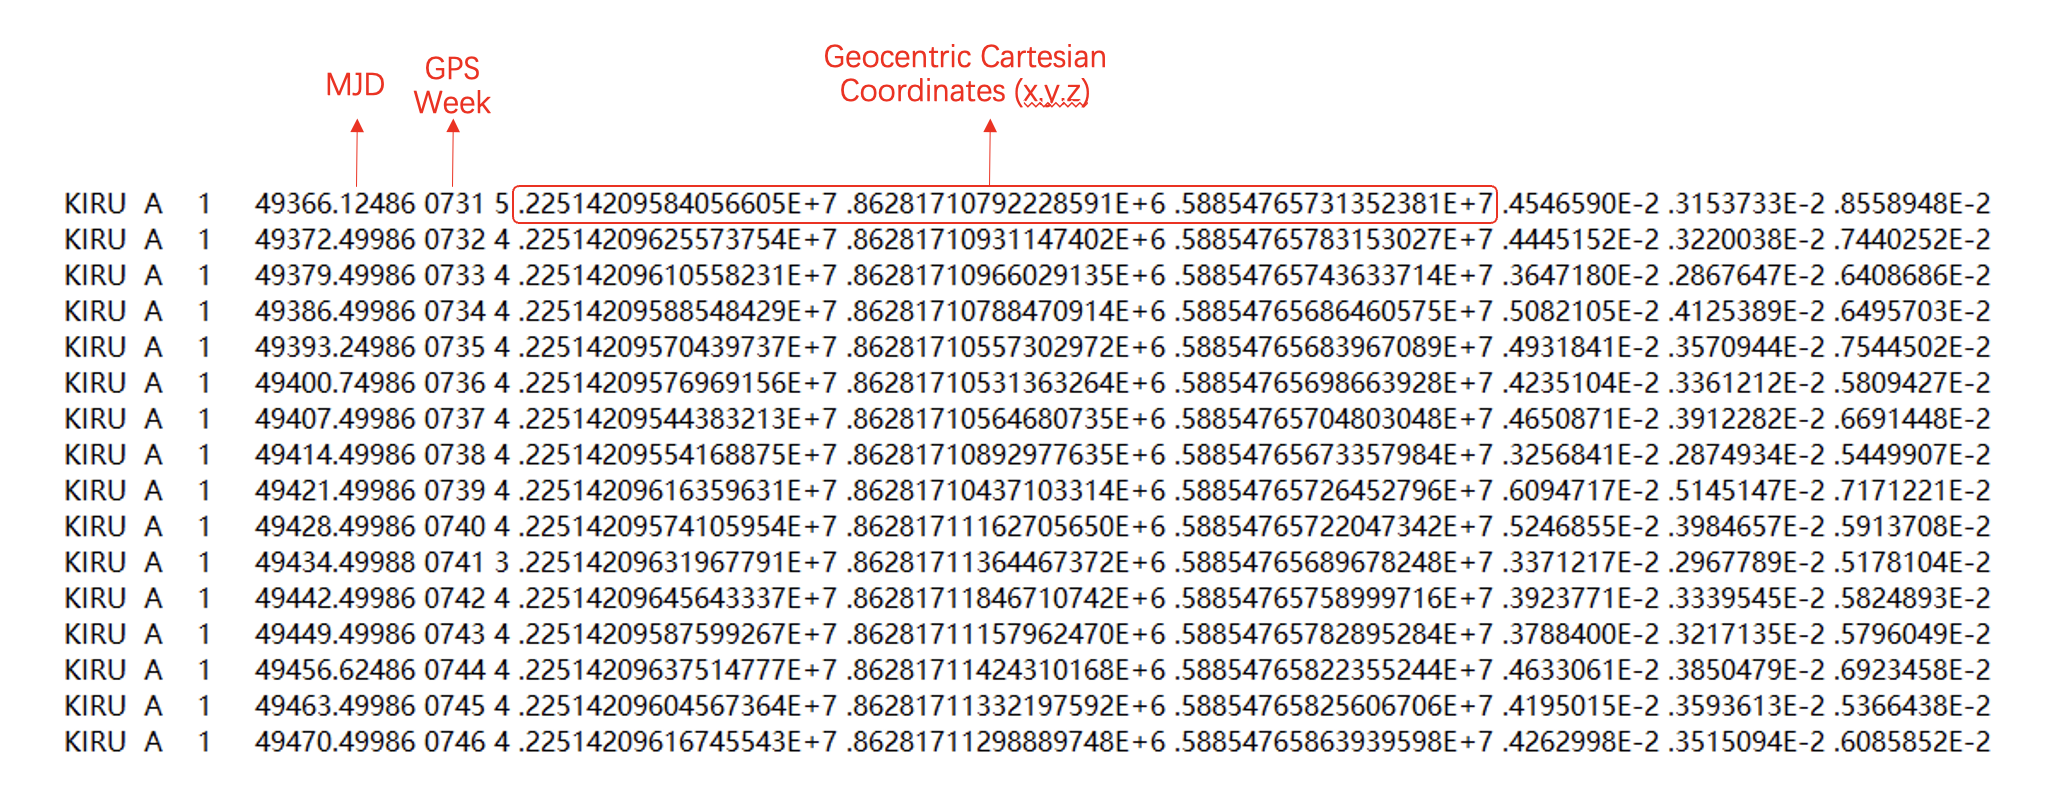
\includegraphics[width=12cm]{./source/xyz.png}
    \caption{station.xyz Description}
    \label{fig:XYZ_obs}
\end{figure}

And the file Discontinuities\_snx provides the discontinuity information in the positions' time series. The reasons for that include change of antenna and receiver, earthquake and so on.
In this example(station: REYK), the discontinuity happened three times due to earthquake, antenna change and unknown reason.
\begin{figure}[htbp]
  \centering
  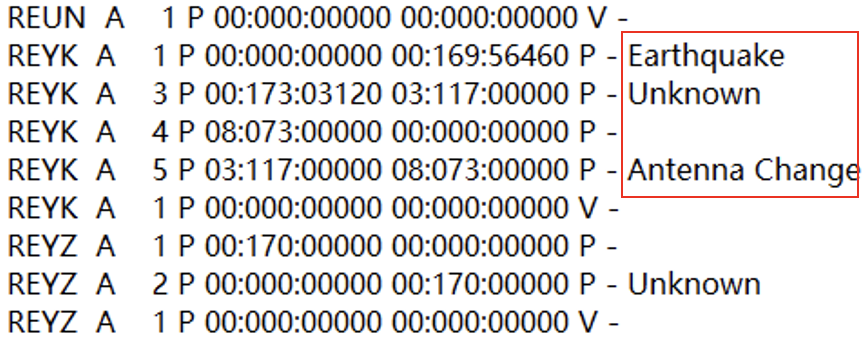
\includegraphics[width=9cm]{../source/dis.png}
  \caption{Discontinuities in time series}
  \label{fig:Dis_snx}
\end{figure}

\subsection{NUVEL 1A Model}
NUVEL(Northeast University Velocity) is a the collective term for geophysical Earth models that describes observable
continental movements through a dynamic theory of plaet tectonics.

The "NNR\_NUVEL1A.txt" gives the rotation referred to epoch $t_0$. 
The file contains the following data, where the leftmost column represents the station name, 
and in that row, the angular velocity changes in three directions are provided (unit: radians per million years or $rad/My$).
\begin{figure}[htbp]
    \centering
    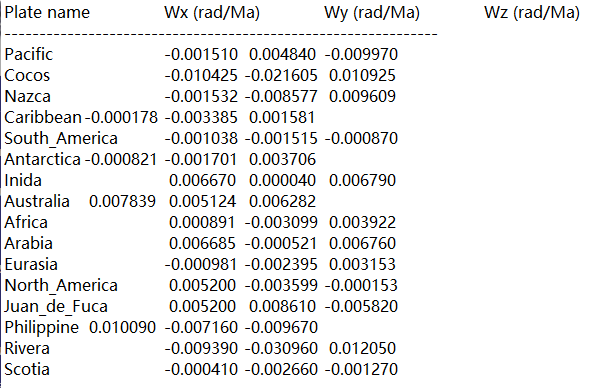
\includegraphics[width=9cm]{../source/nuvel.png}
    \caption{NUVEL\_1A.txt Description}
    \label{fig:Nuvel-1A}
\end{figure}

\subsection{Other data}
\noindent coast30.mat: coast lines for visualization

\noindent crust\_ICE4G.mat, crust\_ICE5G.mat: Global grids with vertical crustal deformations rates [mm/year].
These matrices are given from $89.5^{\circ}$ to $-89.5^{\circ}$ ellipsoidal latitude and $0.5^{\circ}$ to $359.5^{\circ}$ longitude.

\subsection{Matlab Code}

\section{Methodology}
\subsection{Transoformation to LHS}
[Geocentric cartesian coordinate system] is a three-dimensional, earth-centered reference system in which locations are identified by their x, y, and z values. 
The x-axis is in the equatorial plane and intersects the prime meridian (usually Greenwich). 
The y-axis is also in the equatorial plane; it lies at right angles to the x-axis and intersects the 90-degree meridian. 
The z-axis coincides with the polar axis and is positive toward the north pole. The origin is located at the center of the sphere or spheroid.

[Local horizontal system] uses the Cartesian coordinates(East,Nort,Up) to represent position relative to a local origin. The local origin is described by the geodetic coordinates.

The initial coordinates are in the geocentric Cartesian coordinate system and need to be transformed into representation in the local horizontal coordinate system.
In this project, we use two angles and the ITRF2008 point positions as the original point, 
\begin{figure}[htbp]
  \centering
  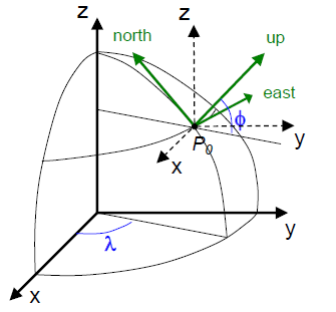
\includegraphics[width=6cm]{../source/transform.png}
  \caption{Coordinates Transformation}
  \label{fig:2lhs}
\end{figure}

Calculate the angle according to stations' geodetic coordinates:

$$\lambda=\arctan\frac{y}{x}$$ 
$$\varphi=\arctan\frac{2}{\sqrt{x^{2}+y^{2}}}$$

Then we can get the rotation matrix:
$$R_2(\delta)=\begin{pmatrix}\cos\delta&0&-\sin\delta\\0&1&0\\\sin\delta&0&\cos\delta\end{pmatrix}\quad R_3(\delta)= \begin{pmatrix}\cos\delta&\sin\delta&0\\-\sin\delta&\cos\delta&0\\0&0&1\end{pmatrix}$$

Transformation of coordinates:
$$\left.\begin{pmatrix}x_{up}\\x_{east}\\x_{north}\end{pmatrix}=R_2(-\varphi^0)R_3(\lambda^0)\left(\begin{pmatrix}x_1\\x_2\\x_3\end{pmatrix}\right.-\begin{pmatrix}x_1^0\\x_2^0\\x_3^0\end{pmatrix}\right)$$

$x^0$are the stations' geodetic coordinates, and $x$ is observations in file '.xyz'.
Notice that we also can directly use the longitude and latitude of stations provided in the file "Discontinuities\_CONFIRMED.snx".

In terms of velocity, its transformation into LHS only requires multiplication by a rotation matrix.
\subsection{Least Square Adjustment for Parameters Estimation}
For time series, $$ y(t)=\beta_{1}+\beta_{2}t+\beta_{3}\mathrm{cos}\omega t+\beta_{4}\mathrm{sin}\omega t $$
among which $\beta_3$ and $\beta_4$ are total amplitude of annual, and $\beta_2$ is linear trend; so we can build model like:
$$\begin{pmatrix}y(t_1)\\\vdots\\y(t_n)\end{pmatrix}=\begin{pmatrix}1&t_1&\cos\omega t_1&\sin\omega t_1\\\vdots&\vdots&\vdots&\vdots\\1&t_n&\cos\omega t_n&\sin\omega t_n\end{pmatrix}\begin{pmatrix}\beta_1\\\beta_2\\\beta_3\\\beta_4\end{pmatrix}$$
We can simppfit the model like: $$Y=X\beta+\varepsilon$$
where $Y$ is the observations, $X$ is the design matrix, $\beta$ is the parameters, and $\varepsilon$ is the noise.

According to least square, minimize the noise, 
derivative the square of noise and set it to zero so we get:
$$\beta=(X^TX)^{-1}X^TY$$ through this we can get the estimated parameters.

\subsection{Model of Plate Tectonics}
The movement of any plate on a spherical Earth can be described through a rotation around the Euler pole:
$$\underline{\Omega}=(\Omega_{1},\Omega_{2},\Omega_{3})^{T}$$
In point $\underline{x}_{0}=(x,y,z)^{T}$ the velocity vector v is obtained by:
$$\underline{v}=\underline{\Omega}\times\underline{x}_0=\begin{pmatrix}0&&-\Omega_z&&\Omega_y\\\Omega_z&&0&&-\Omega_x\\-\Omega_y&&\Omega_x&&0\end{pmatrix}\begin{pmatrix}x\\y\\z\end{pmatrix}$$

\subsection{Program Description}

\section{Results and Analysis}
\subsection{Time Series, Linear Trend and Residuals}
Through the least square adjustment, out group get the time series of these three stations as shown below:
\begin{figure}[htbp]
  \centering
  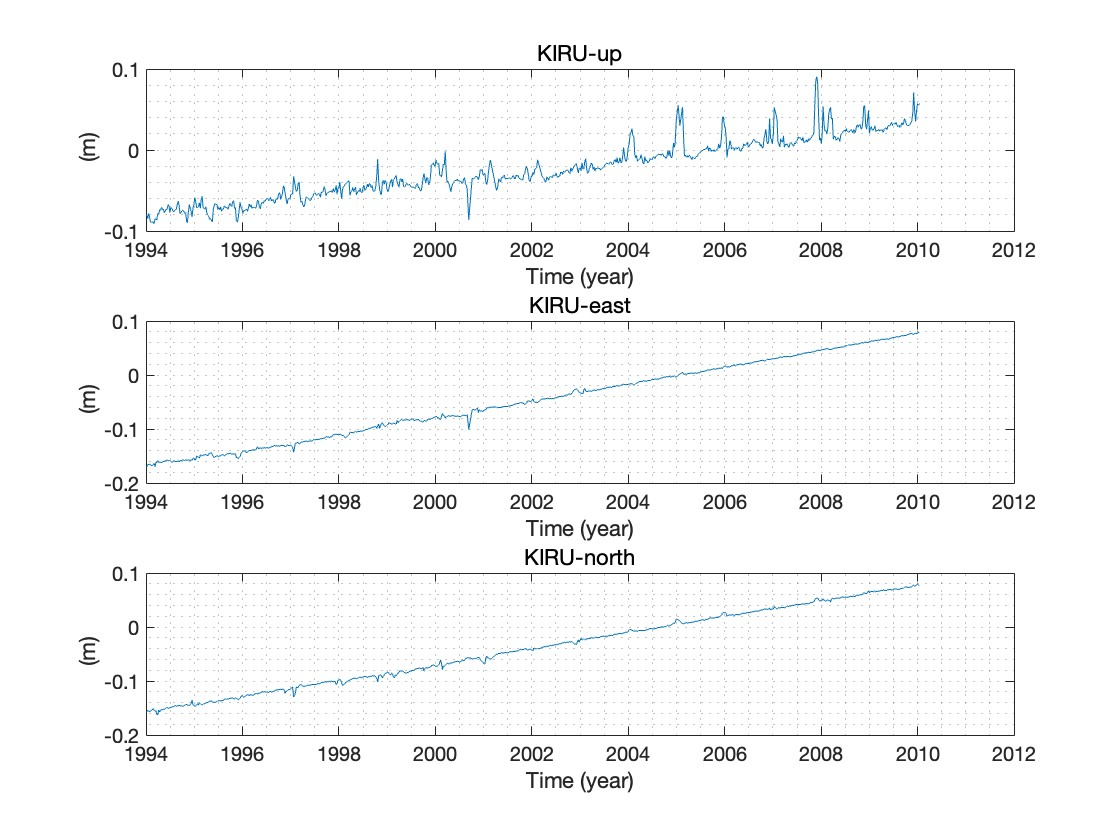
\includegraphics[width=11cm]{../result/re_figure/fig_kiru/5.jpg}
  \captionsetup{skip=0.2cm}
  \caption{Time Series of KIRU/(meter)}
  \label{fig:Ori_KIRU}
\end{figure}
\begin{figure}[htbp]
  \centering
  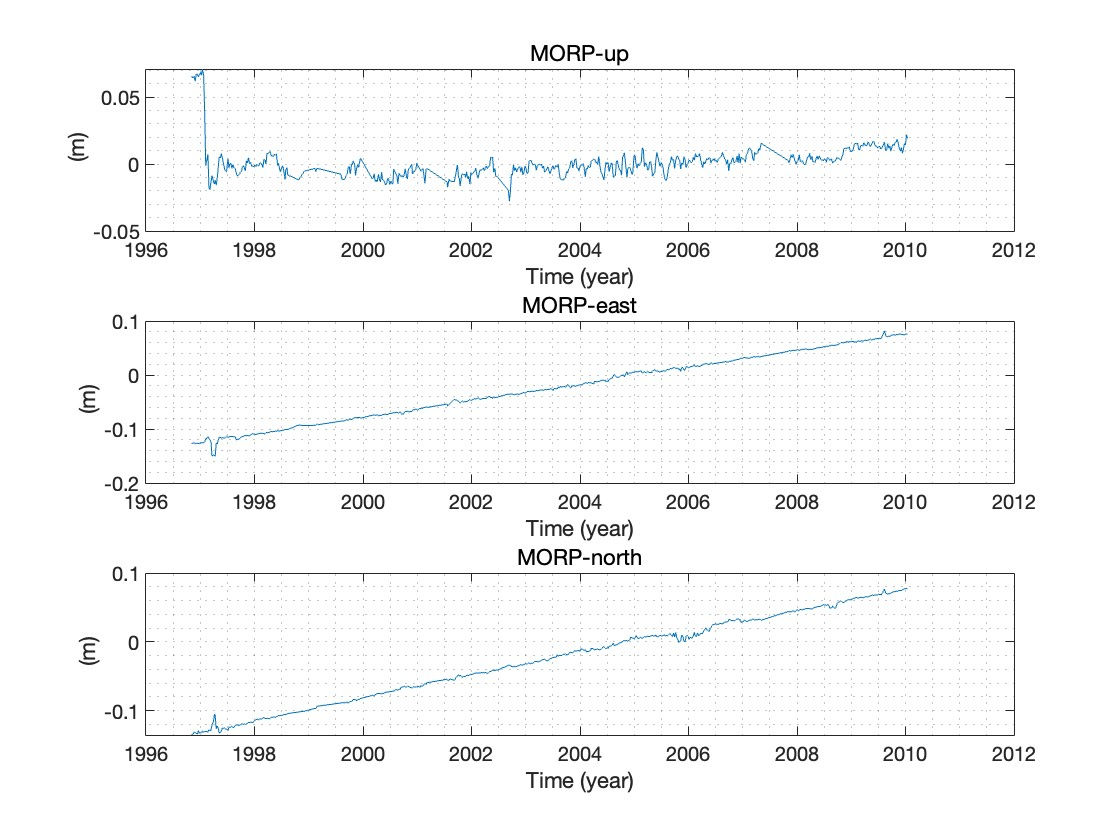
\includegraphics[width=11cm]{../result/re_figure/fig_MORP/5.jpg}
  \caption{Time Series of MORP(meter)}
  \label{fig:Ori_MORP}
\end{figure}
\begin{figure}[htbp]
  \centering
  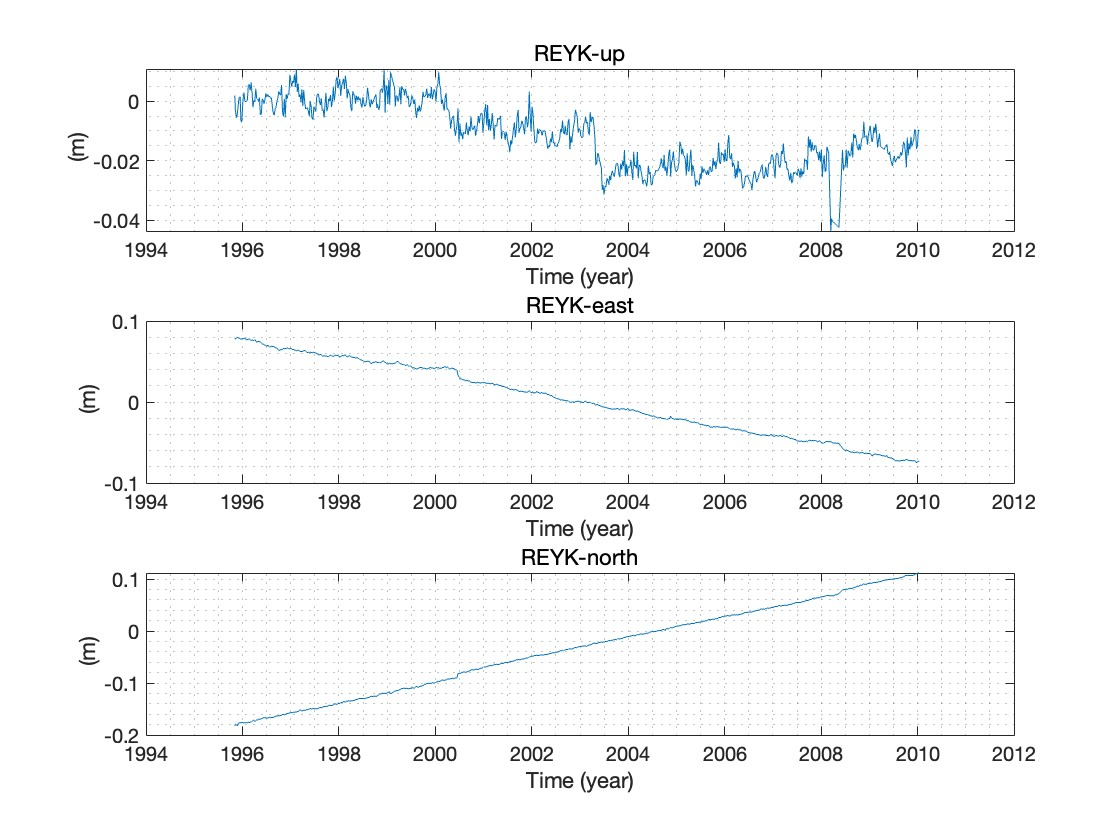
\includegraphics[width=11cm]{../result/re_figure/fig_REYK/figure1.jpg}
  \caption{Time Series of REYK(meter)}
  \label{fig:Ori_REYK}
\end{figure}

And we can see that the linear trend (millimeter per year) of KIRU in Up, East and North directions are 7.3089, 15.5296 and 14.8375 respectively, 
 that of MORP in Up, East and North directions are 0.4201, 15.5923 and 15.9229 respectively,
 and as for REYK, the linear trend in Up, East and North directions are ,  and  respectively.
 \vspace{5pt}
\begin{table}[H]
  \centering
  \caption{Linear Trend of Time Series}
    \begin{tabular}{lrrr}
    \large Station & \multicolumn{3}{c}{\large Linear Trend(mm/y)} \\
    \midrule
          &\multicolumn{1}{l}{\large UP} & \multicolumn{1}{l}{\large EAST} & \multicolumn{1}{l}{\large NORTH} \\ [5pt]
          
     KIRU&7.3089 & 15.5296 & 14.8375\\[3pt]
     MORP&0.4201 & 15.5923 & 15.9229\\ [3pt]
     REYK&-2.0306 & -10.9442 & 20.6032\\
    \end{tabular}%
  \label{Tab:lin_trend}%
\end{table}

After we minus the linear trend, out group get the residual time series of these three stations as below 
and the specific vaules are shown in the table 1. 
At the same time, table 2 shows the total amplitude of non-linear trend (millimeter per year) which can be computed by $\sqrt{\beta_3^2+\beta_4^2}$.

When we removing the linear trend, our group also remove the constant term in the model($\beta_1 + \beta_2 t$), 
so that we can see more clearly about the residaul values.
After doing this, we can see residual value in millimeter in three directions of three stations.
\begin{figure}[H]
  \centering
  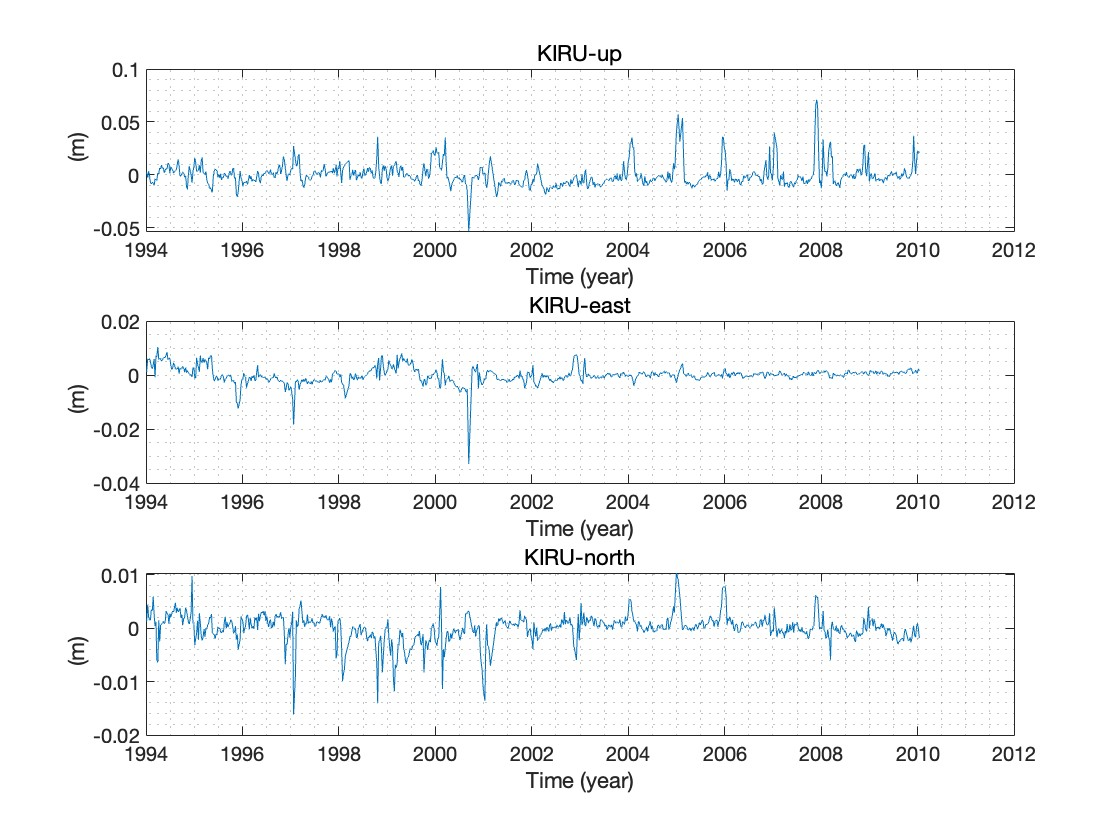
\includegraphics[width=11cm]{../result/re_figure/fig_kiru/4.jpg}
  \captionsetup{skip=0.2cm}
  \caption{Residual Time Series of KIRU}
  \label{fig:Res_KIRU}
\end{figure}
\begin{figure}[H]
  \centering
  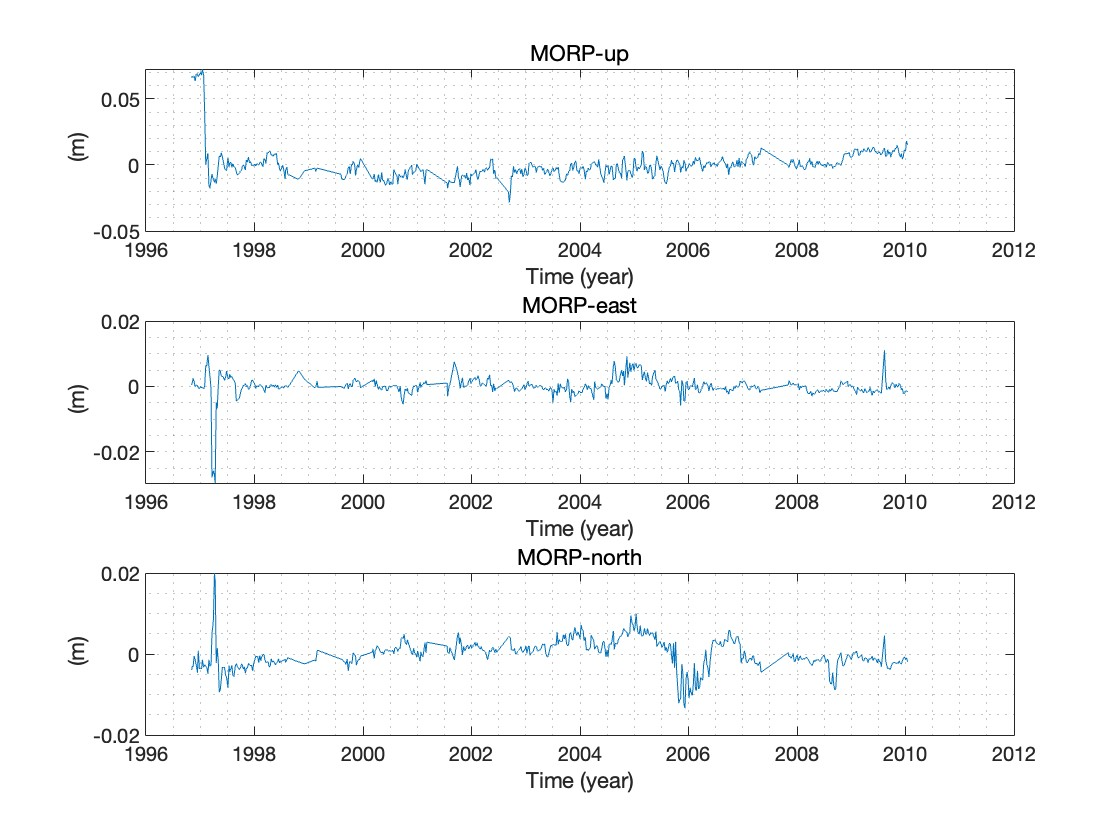
\includegraphics[width=11cm]{../result/re_figure/fig_MORP/4.jpg}
  \caption{Residual Time Series of MORP}
  \label{fig:Res_MORP}
\end{figure}
\begin{figure}[H]
  \centering
  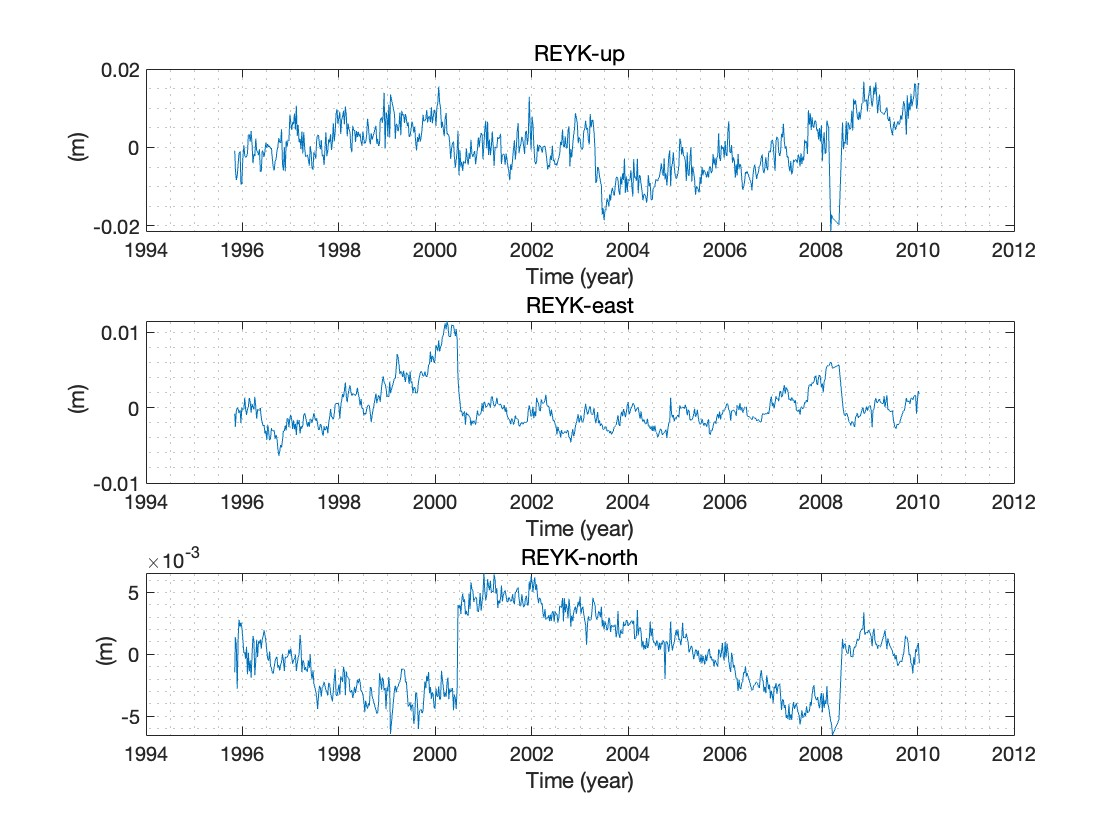
\includegraphics[width=11cm]{../result/re_figure/fig_REYK/figure2.jpg}
  \caption{Residual Time Series of REYK}
  \label{fig:Res_REYK}
\end{figure}

Due to the discontinuities in the observations, our group using the differnet reference coordinates in time series given by the file "Discontinuities\_CONFIRMED.snx". 
After separat modeling of different parts of time seies, we can get the residual time series of these three stations as below, where we use different colors to represent different parts:
\begin{figure}[H]
  \centering
  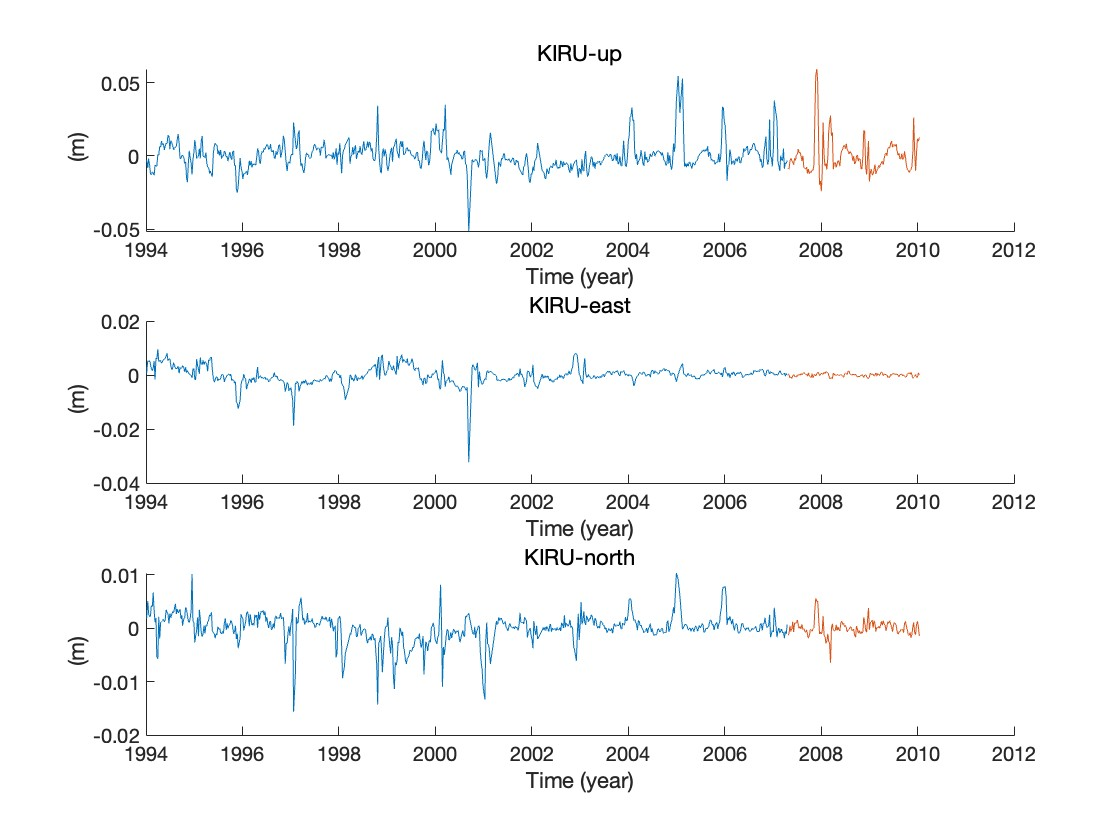
\includegraphics[width=11cm]{../result/re_figure/fig_kiru/3.jpg}
  \captionsetup{skip=0.2cm}
  \caption{Modified Residual Time Series of KIRU}
  \label{fig:nRes_KIRU}
\end{figure}
\begin{figure}[H]
  \centering
  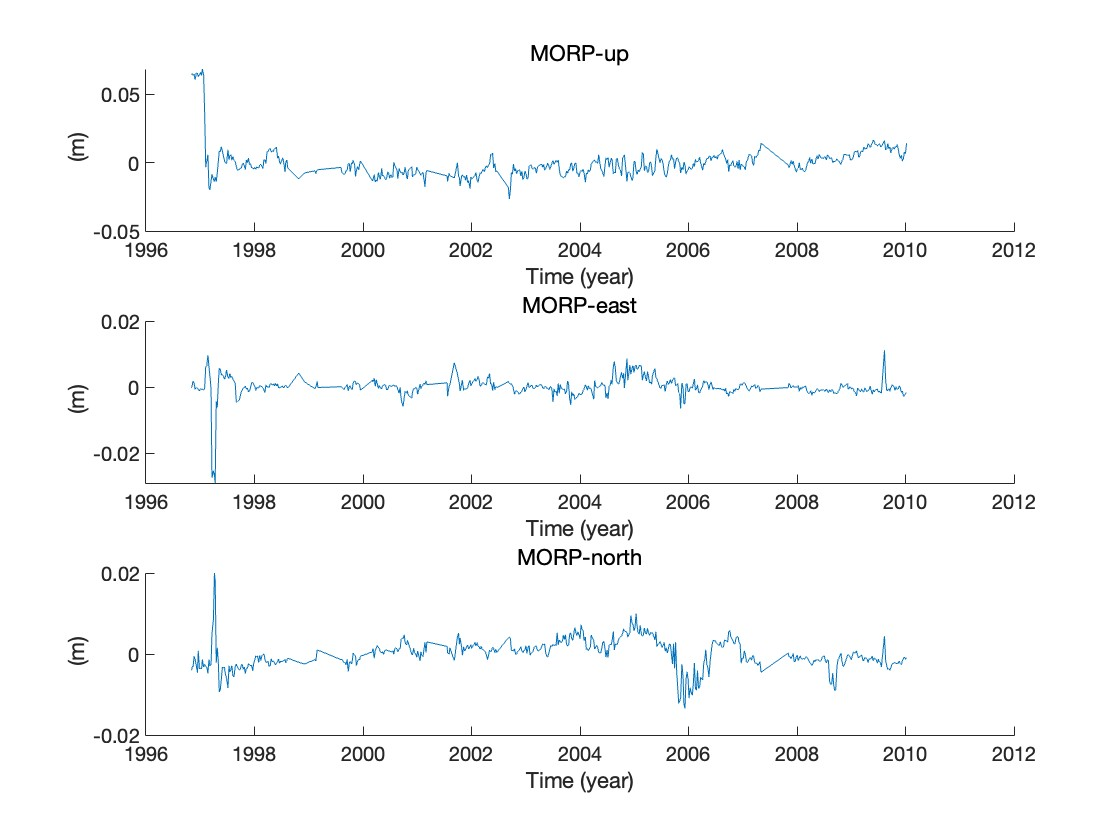
\includegraphics[width=11cm]{../result/re_figure/fig_MORP/3.jpg}
  \caption{Modified Residual Time Series of MORP}
  \label{fig:nRes_MORP}
\end{figure}
\begin{figure}[H]
  \centering
  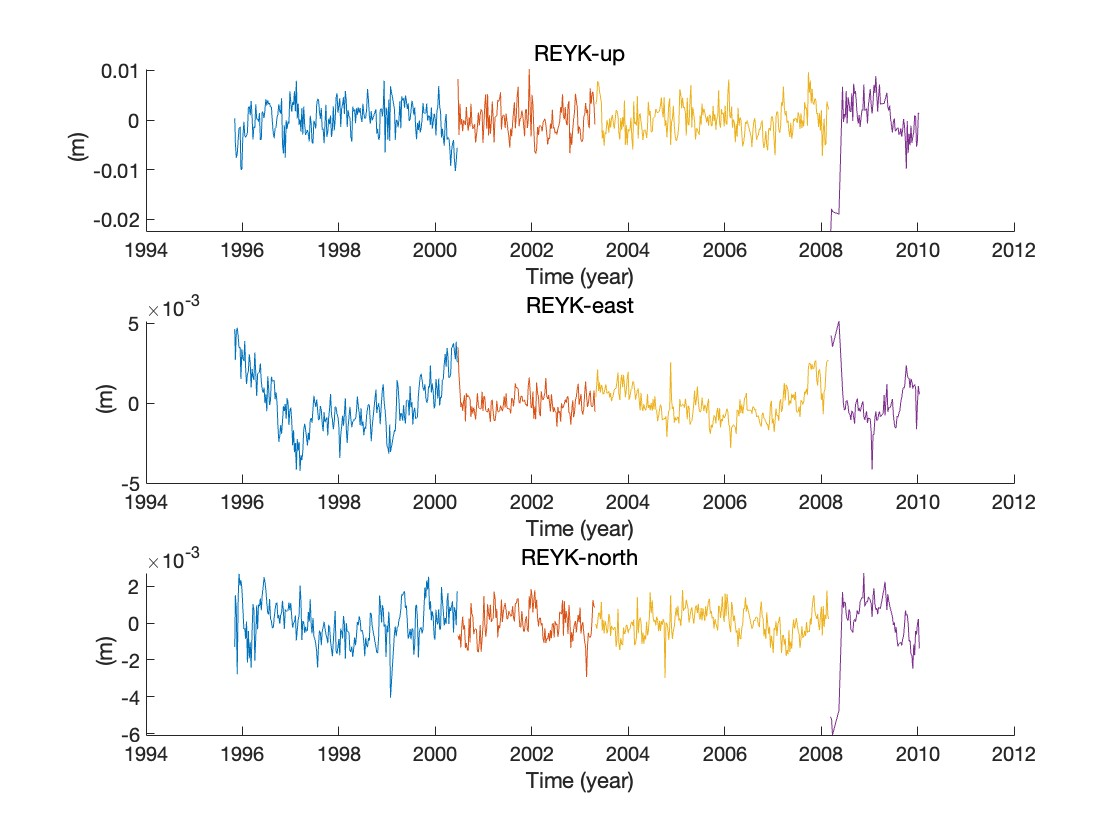
\includegraphics[width=11cm]{../result/re_figure/fig_REYK/figure3.jpg}
  \caption{Modified Residual Time Series of REYK}
  \label{fig:nRes_REYK}
\end{figure}

Obviously, the residual values of UP direction are much larger than the other two directions, which also are predominant in total residual values.
Through, we know that GPS residuals on the three components are dominated by flicker noise.

Meanwhile, our group also found some anomalies in the residual time series. Firstly, we find there is an annual signal in the all time series, 
these signals' amplitude are much large for KIRU, but are small(1-2 millimeter) in MORP and REYK. 
We speculate that the annula signals is caused mainly by the seasonal changes in the atmosphere.
Plus, there are some sudden changes, like the one in 1997 of MORP, the one in 2000 of KIRU and the ones in 2000 and 2008 of REYK.
We supposed that these changes are caused by the discontinuities in the observations and recording errors or instrument malfunction.

Additionally, we also find that the residual time series of MORP are much more stable than the other two stations, 
From the map, it can be observed that MORP has the lowest latitude, so we speculate that this is due to stronger interference received by GPS signals in high-latitude areas, which is related to various factors. 
Firstly, the ionospheric effects are more significant in high-latitude regions. 
Additionally, particles generated by solar activities are attracted toward the Earth's North Pole, causing electromagnetic interference and making GPS signals more unstable. 
Secondly, receivers in high-latitude areas receive satellite signals at lower angles, which increases the atmospheric impact on the signals, meanwhile this also causes receiving signals from fewer satellites. 
Furthermore, much more snow and ice in high-latitude regions strengthens the effects of multipath effect. 
In summary, various factors contribute to a reduction in the accuracy of position measurements in high-latitude areas.


\subsection{Comparison with the Plate Tectonics Model}
Through the NUVEL 1A model, we can get the velocity of three stations, for this model only consider the horizontal movements,
so our group only compare the velocity in East and North directions. 

The comparison is shown below 
and we can see clearly that the horizontal velocities from NUVEL and GNSS observations differ slightly, 
sometimes the differences are even considerable like the one in REYK, where velocities in East directions are opposite:
% three stations each has two subfigures, one global and one local
\begin{figure}[H]
  \centering
  {
  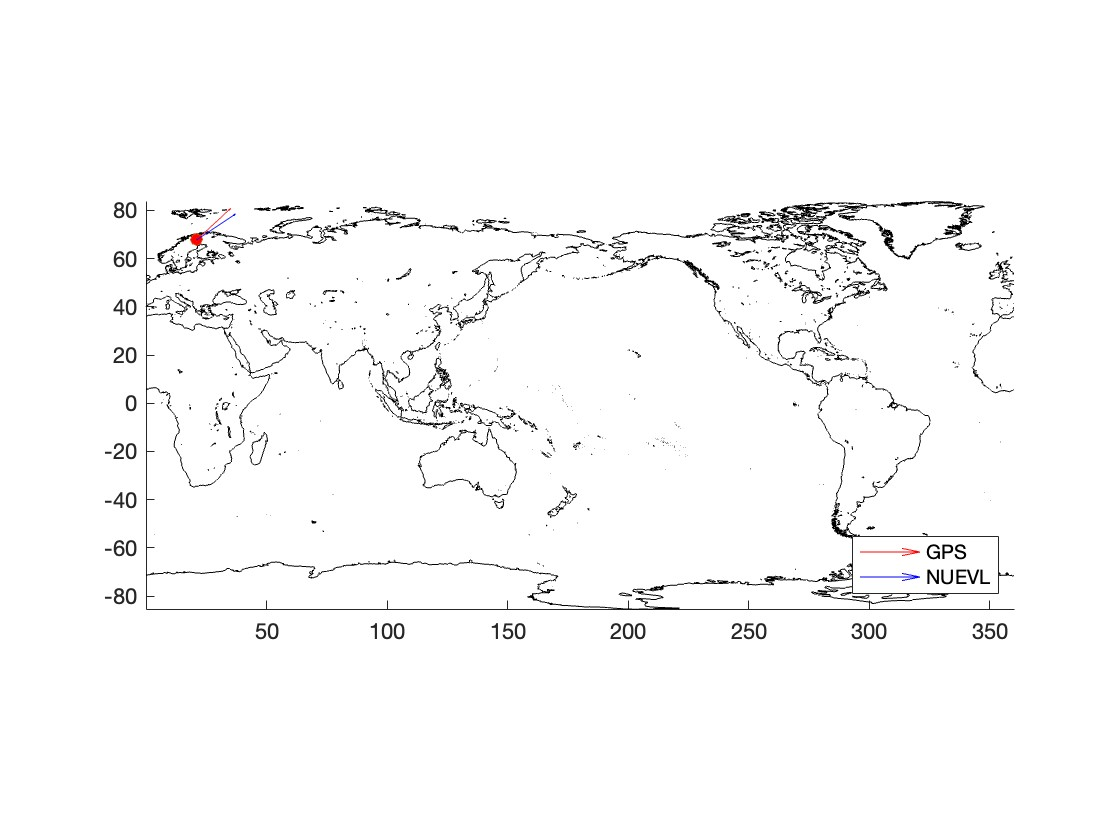
\includegraphics[width=8cm]{../result/KIRU/KIRU_4.jpg}}
  \hspace{3pt}    
  {
  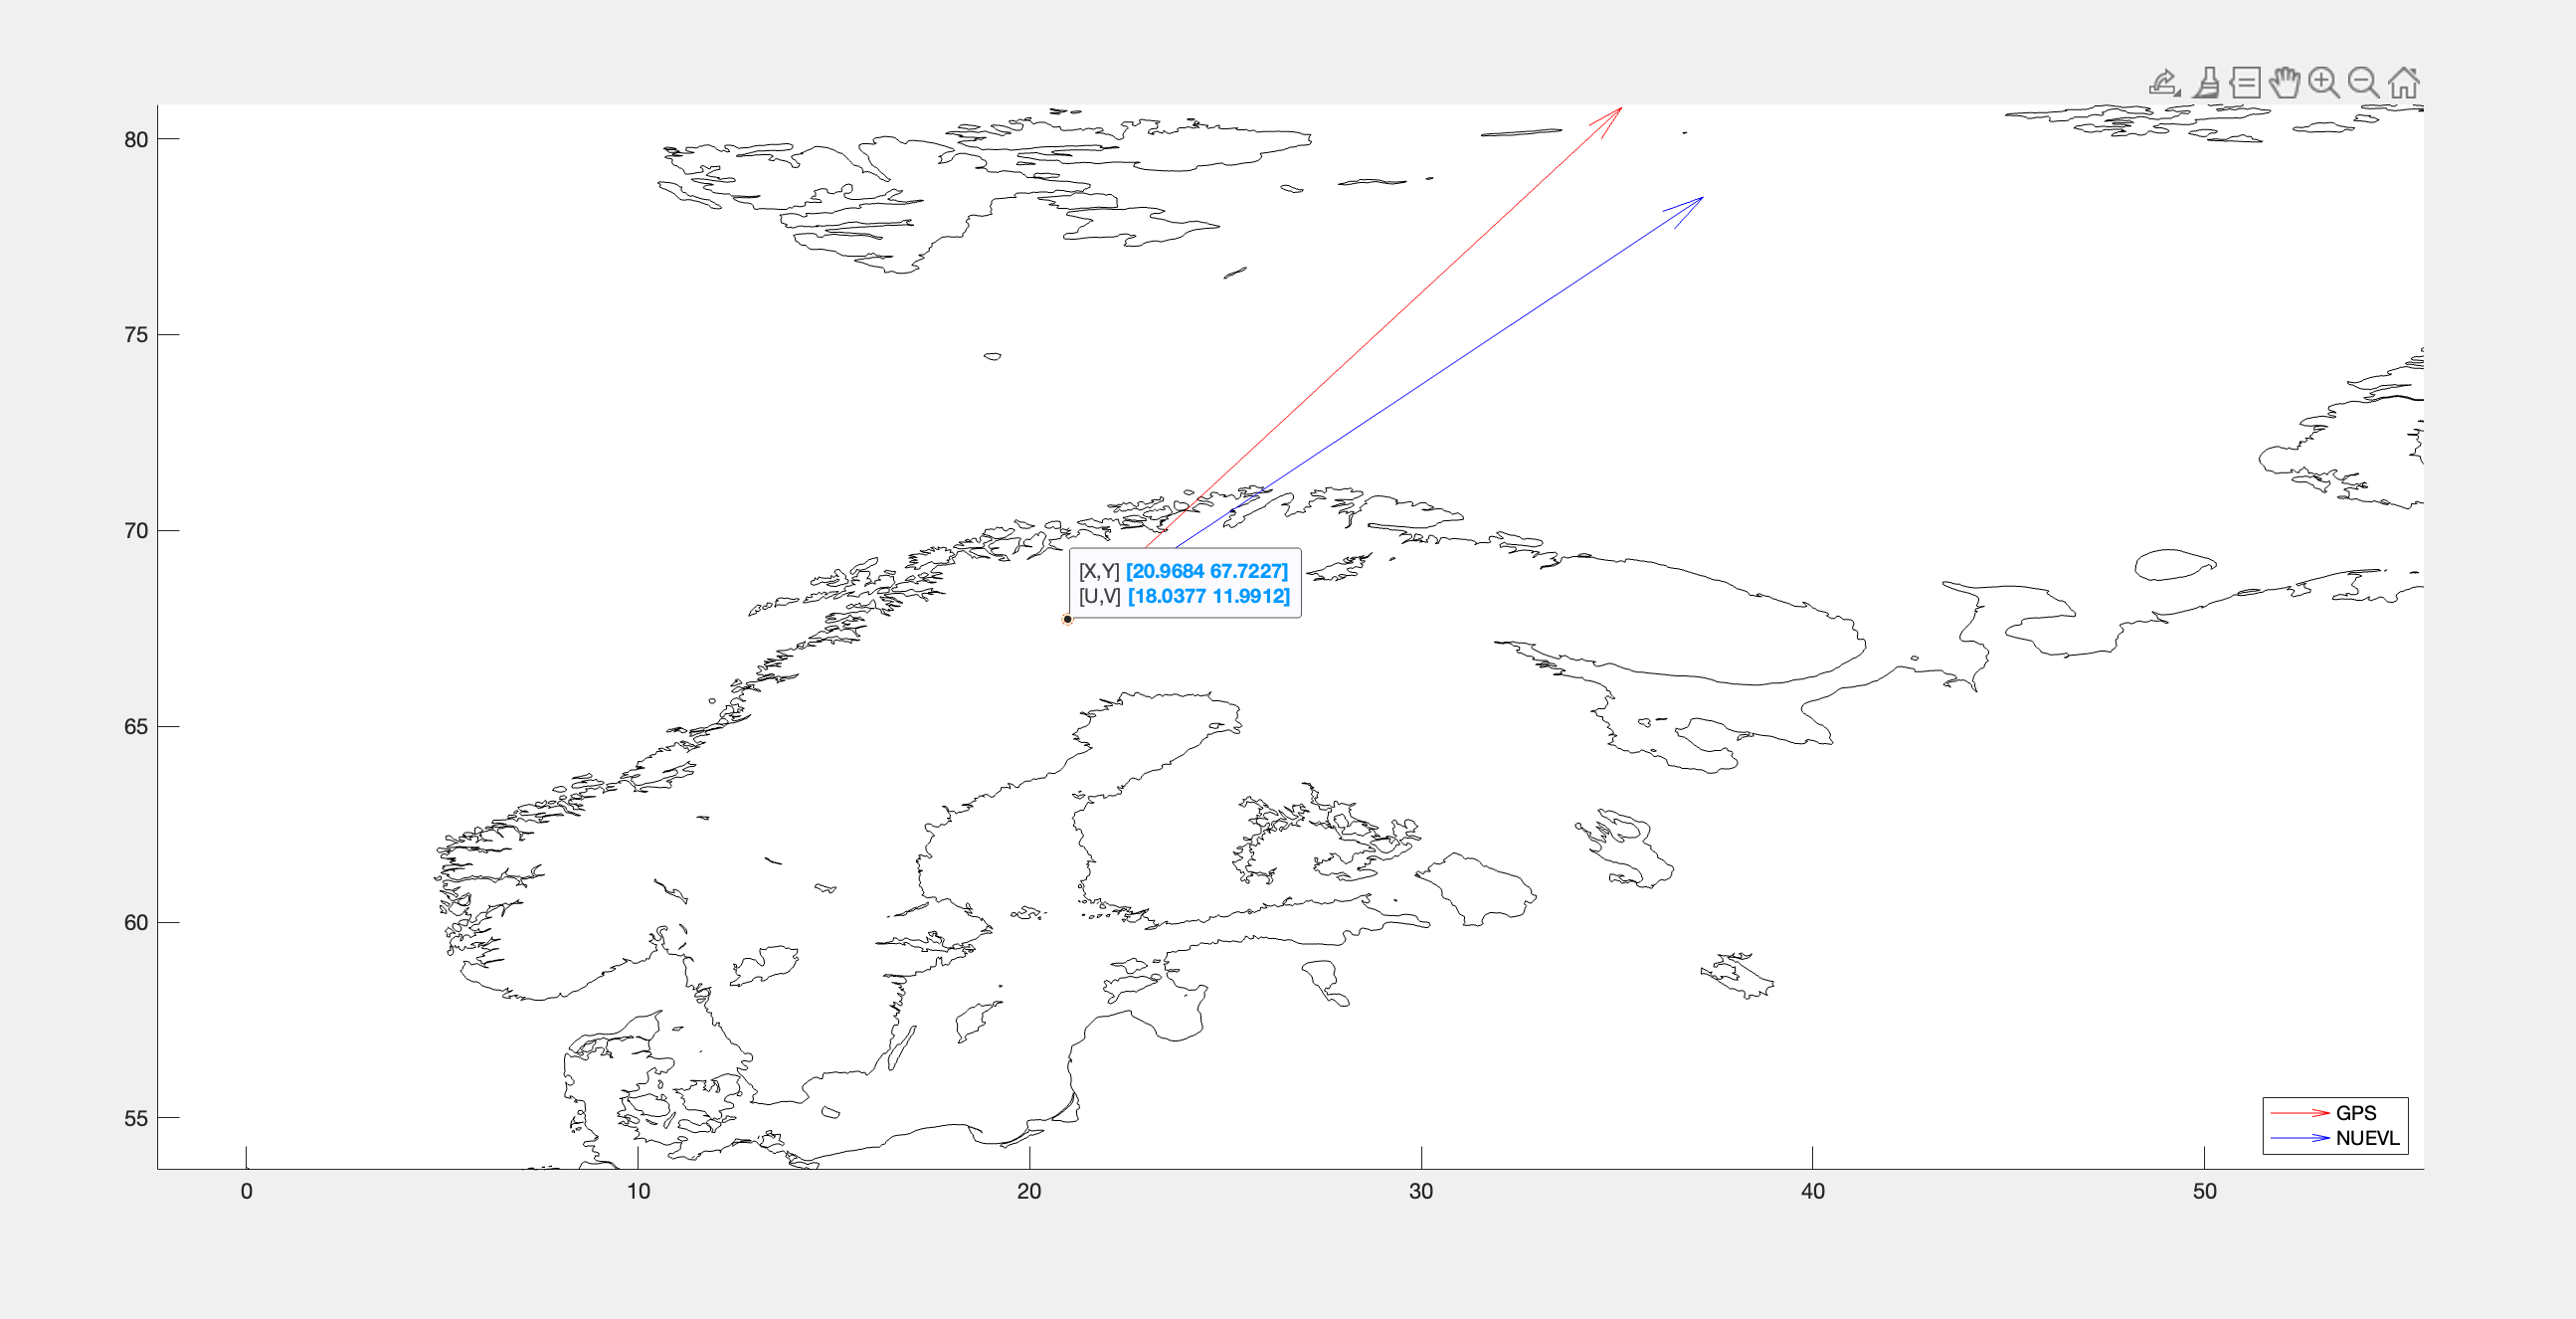
\includegraphics[width=8cm]{../result/KIRU/KIRU_4(zoom_up).jpg}}
  \caption{Horizontal Movements Comparison of KIRU}
  \label{fig:Vel_KIRU}
  \end{figure}
  \begin{figure}[H]
    \centering
    {
    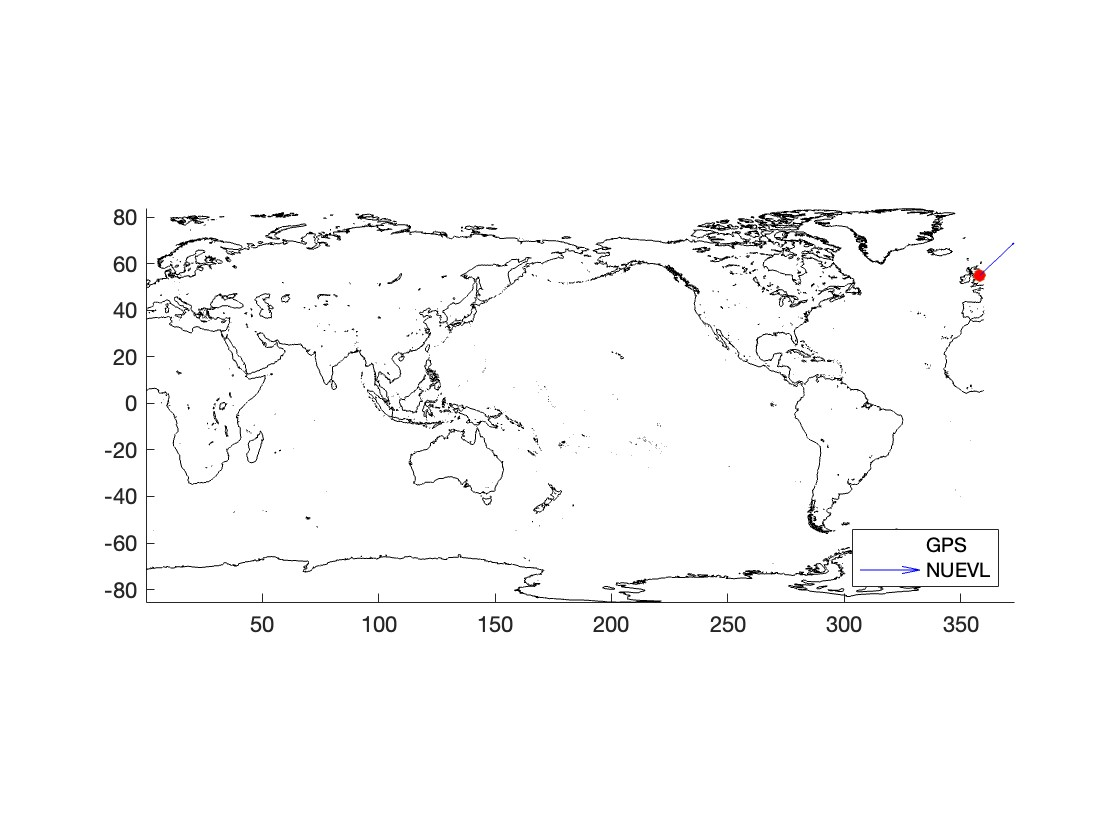
\includegraphics[width=8cm]{../result/MORP/MORP_4.jpg}}
    \hspace{3pt}    
    {
    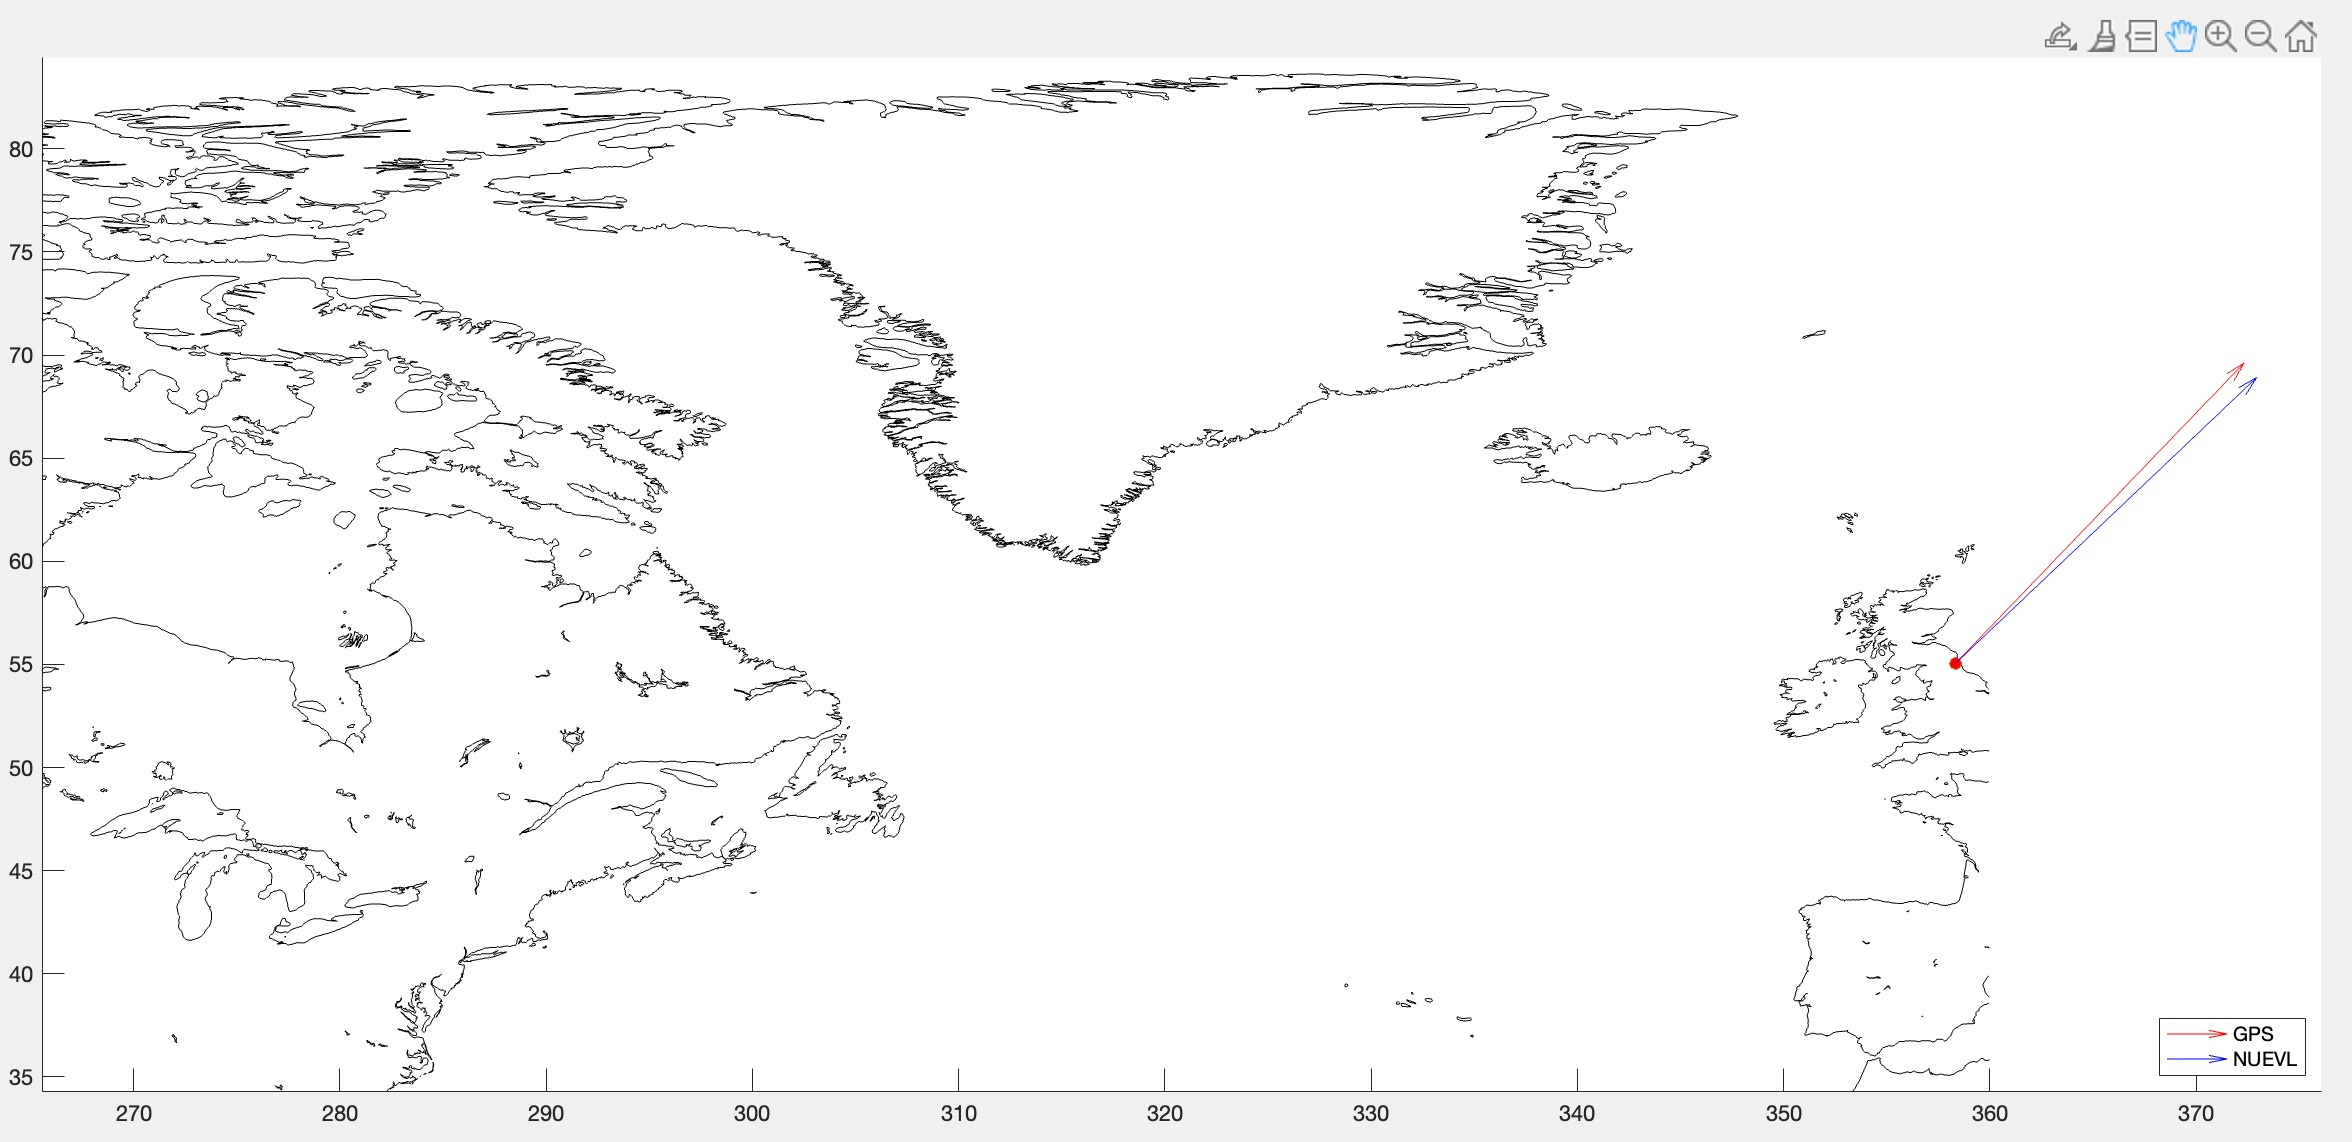
\includegraphics[width=8cm]{../result/MORP/MORP_4(zoom_up).jpg}}
    \caption{Horizontal Movements Comparison of MORP}
    \label{fig:Vel_MORP}
  \end{figure}
  \begin{figure}[H]
    \centering
    {
    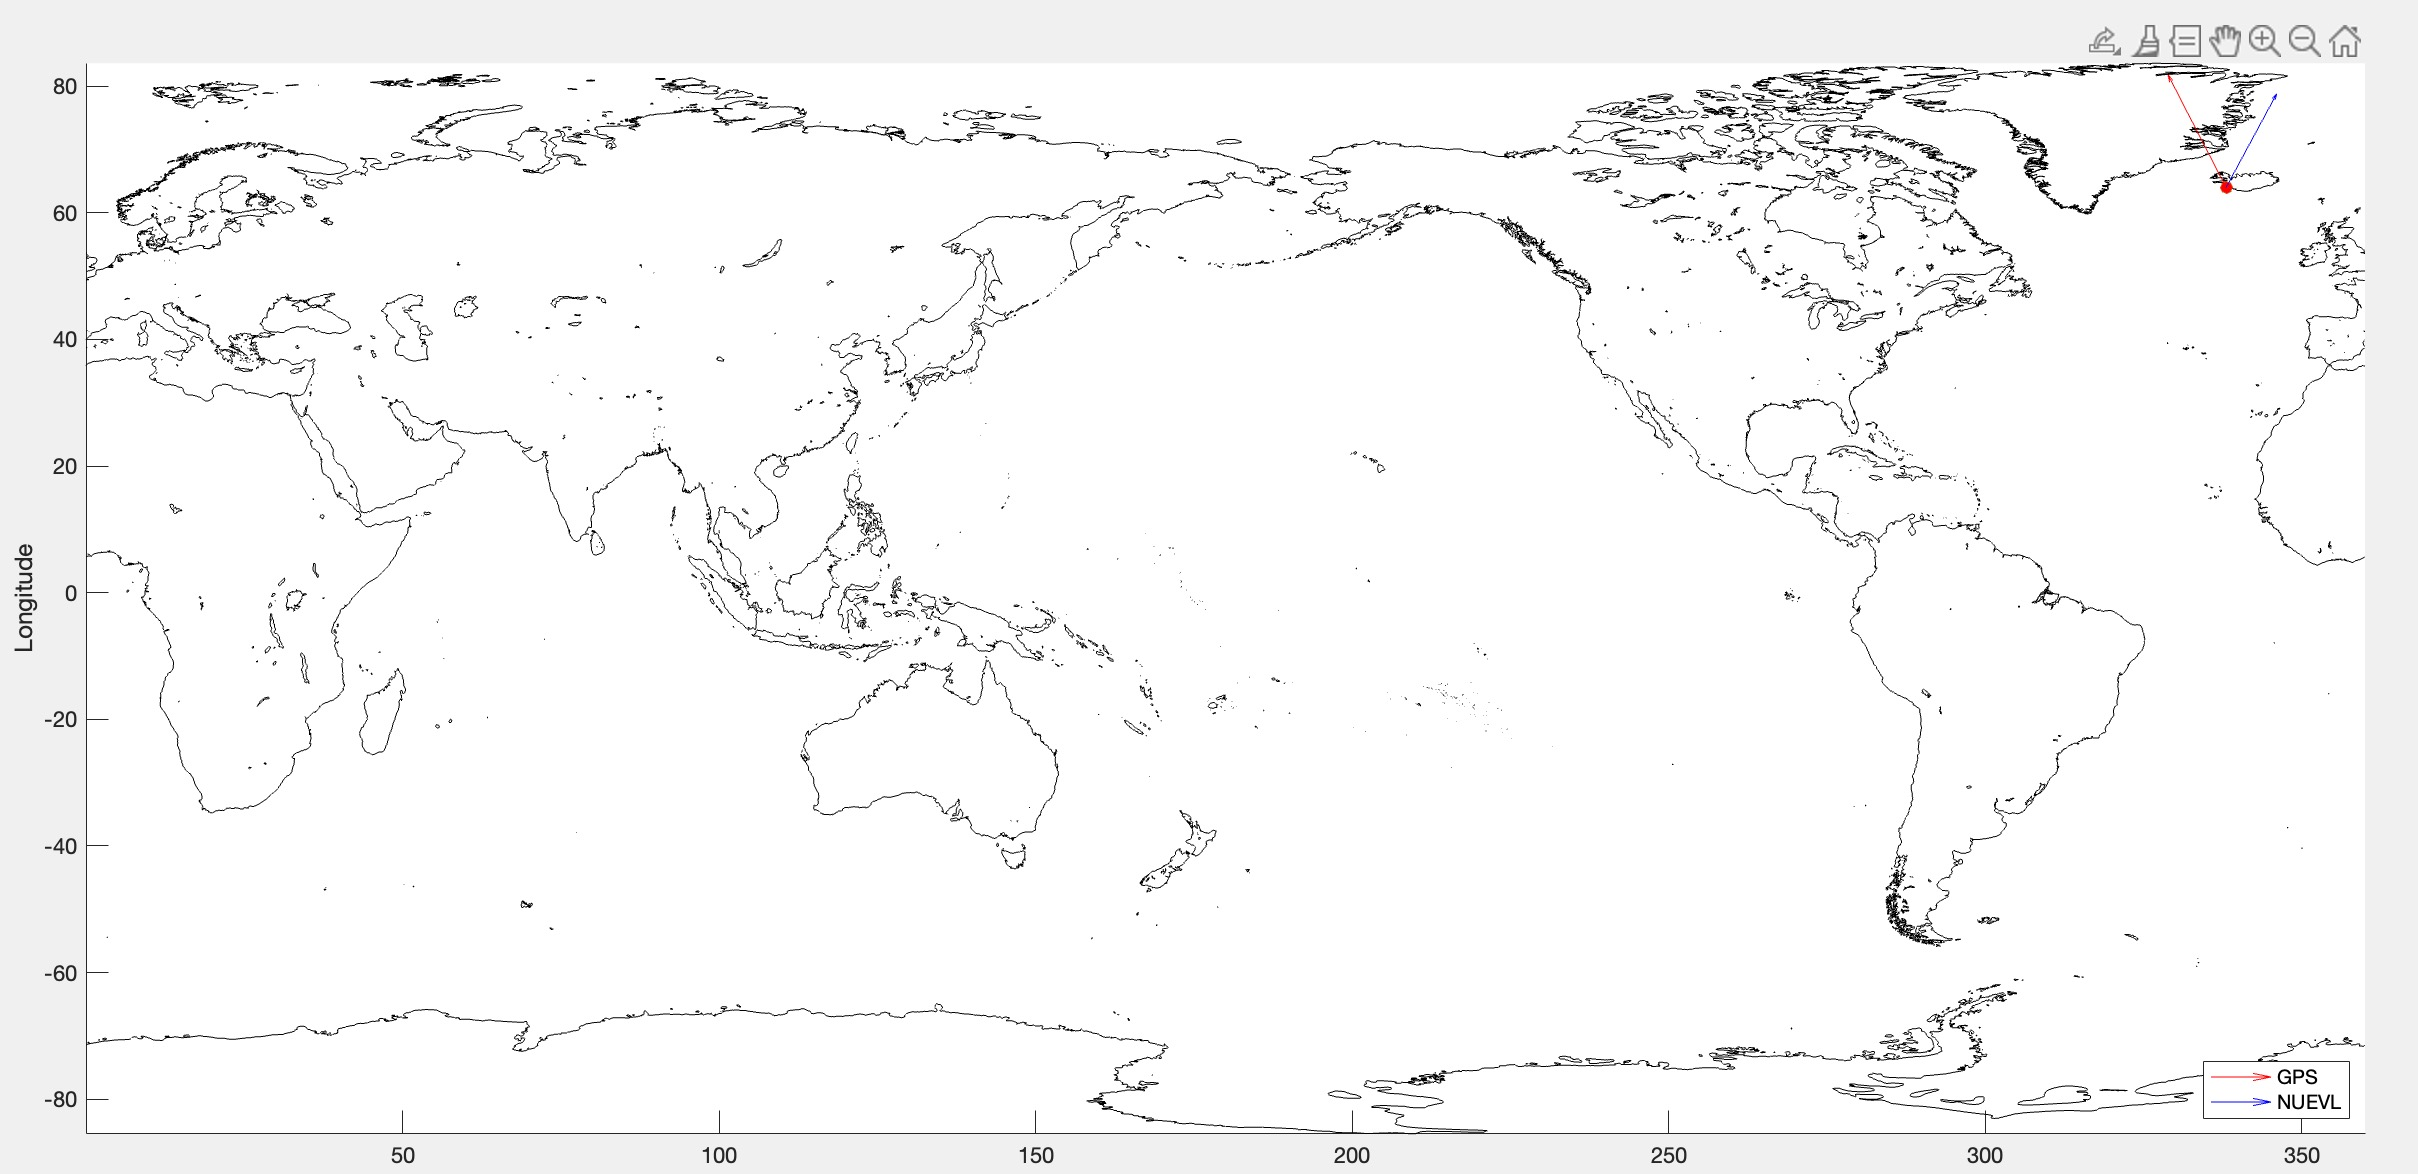
\includegraphics[width=8cm]{../result/re_figure/fig_REYK/截屏/figure4_new.jpg}}
    \hspace{3pt}    
    {
    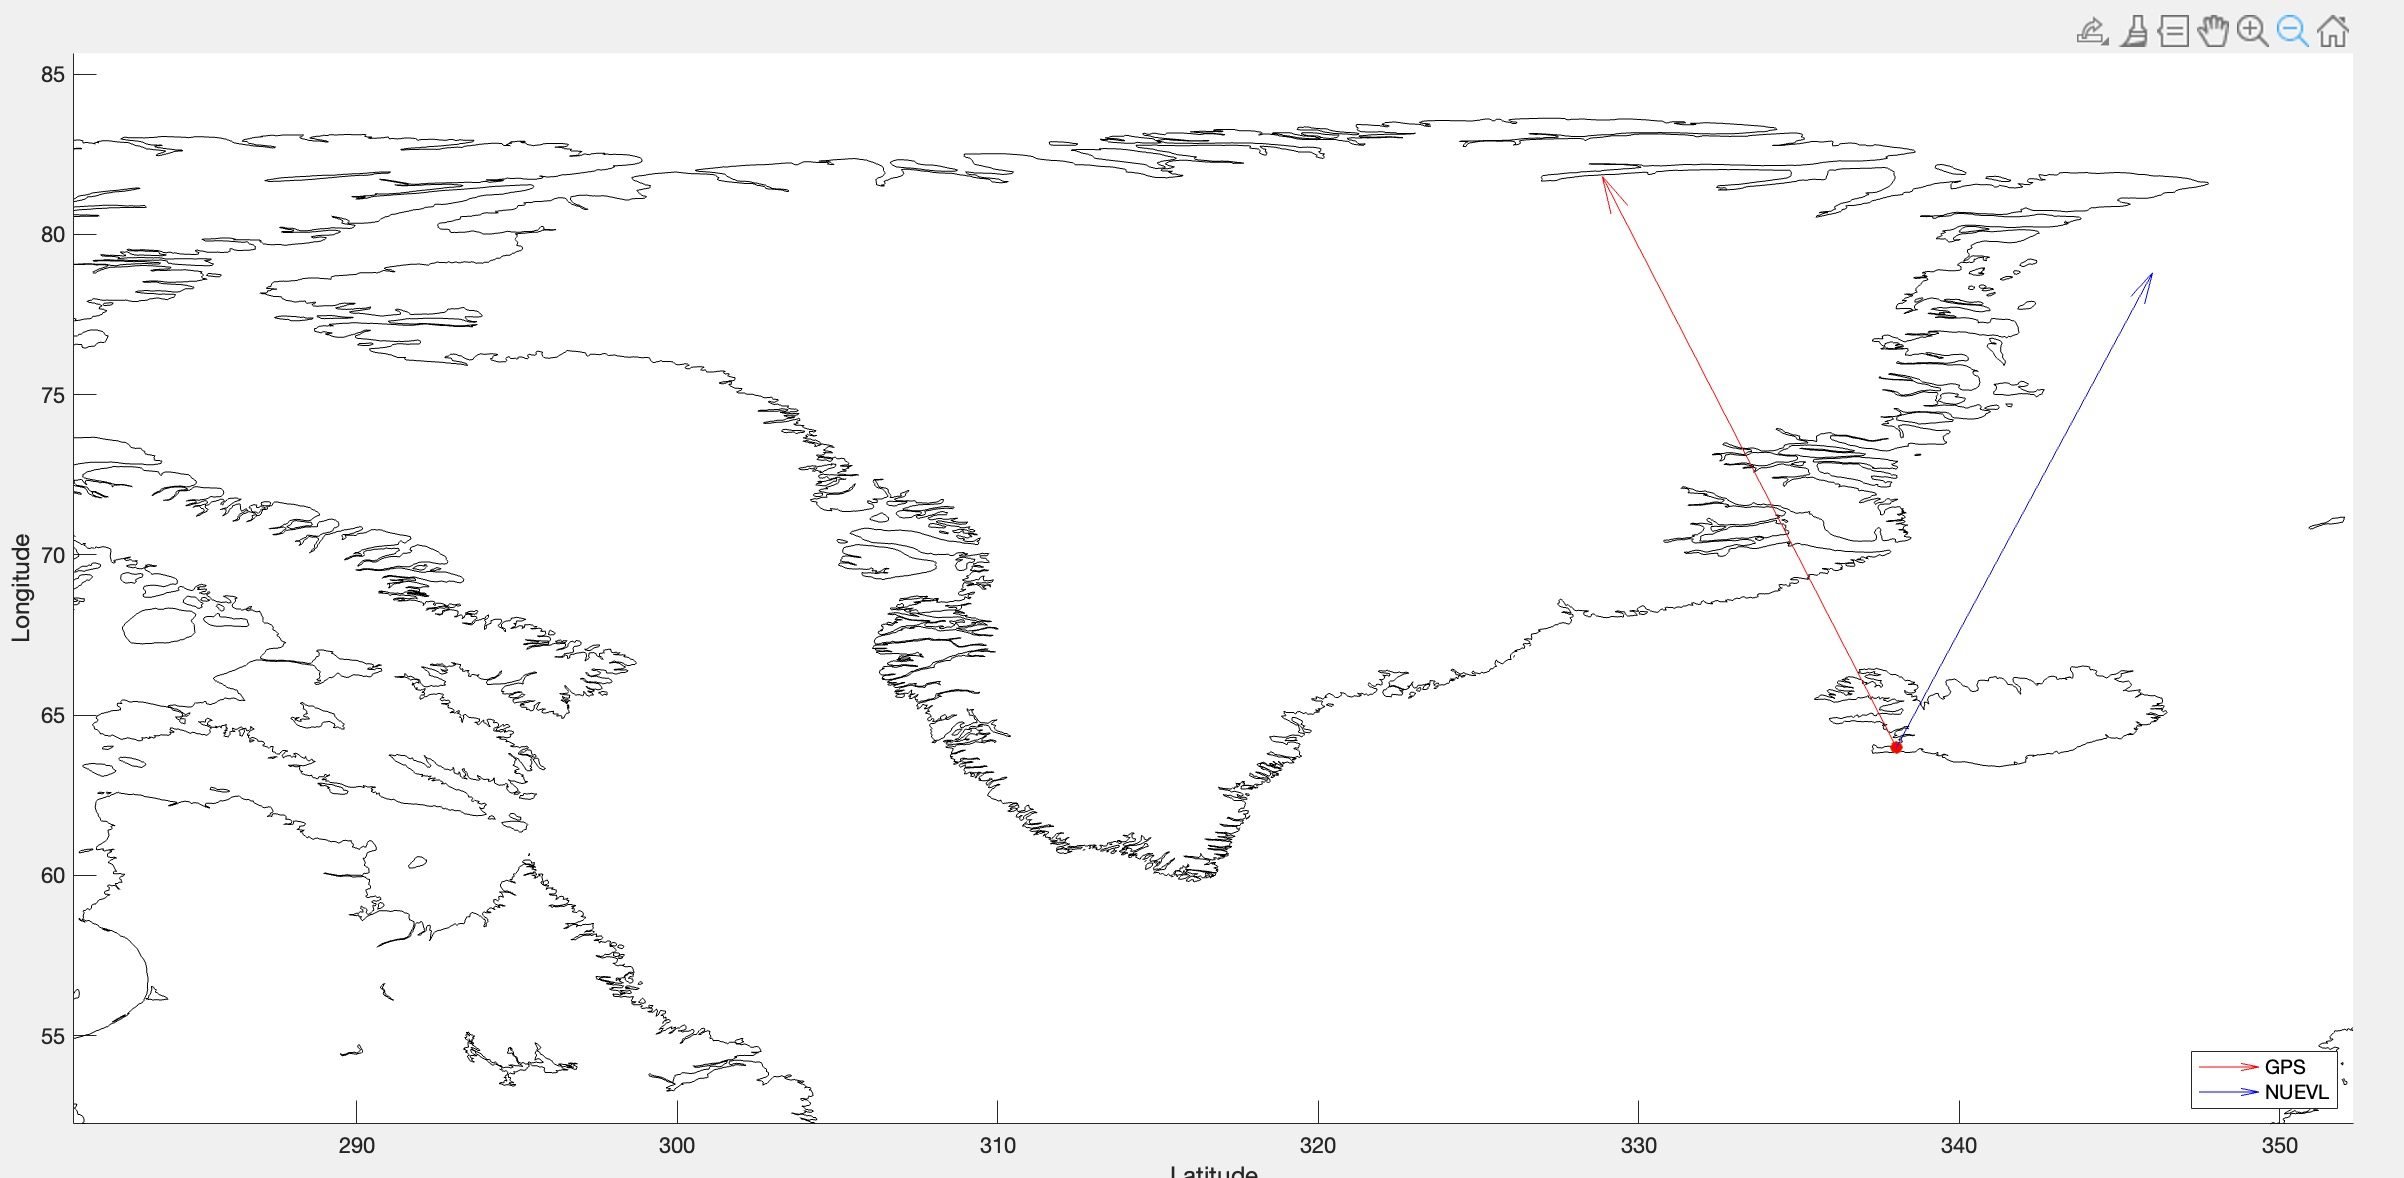
\includegraphics[width=8cm]{../result/re_figure/fig_REYK/截屏/figure4(zoomup).jpg}}
    \caption{Horizontal Movements Comparison of REYK}
    \label{fig:Vel_REYK}
  \end{figure}

And we give the specific values of horizontal velocity(in the East and North axis) as below:
\vspace{6pt}
% Table generated by Excel2LaTeX from sheet 'Sheet1'
\begin{table}[htbp]
  \centering
  \caption{Horizontal Movement Rates}
    \begin{tabular}{ccc|cc}
    \large Station & \multicolumn{4}{c}{\large Horizontal Velocity/(m/y)} \\[5pt]
    \midrule
          & \multicolumn{2}{c}{GNSS Observation} & \multicolumn{2}{c}{NUVEL-1A Model} \\[3pt]
          & EAST  & \multicolumn{1}{c}{NORTH} & EAST  &  NORTH \\[4pt]
    \large KIRU  & 0.0157 & 0.0145 & 0.0180 & 0.0120 \\[4pt]
    \large MORP  &  0.0156 & 0.0159 &  0.0162 & 0.0154 \\[4pt]
    \large REYK  & -0.0104 & 0.0198 &  0.00878 & 0.01646 \\
    \end{tabular}%
  \label{tab:Hori_vel}%
\end{table}%

For the reason that horizontal movements from GNSS observations don't fit very well that from the NUVEL-1A model well,
our group think there are several reasons for this: 
Firstly, both GNSS observations and the data used in the NUVEL model are interfered by various factors. 
The GPS signal and observations are affected by multipath effects and ionospheric interference, 
while seismic activities and receiver changes can also impact the observations. 
Additionally, the NUVEL 1A model has simplified the plate structure and motion, it isn't considered as a highly accurate model now. 
Also, NUVEL model uses data from multiple GNSS observations, 
and there will certainly be some offsets compared to our calculation only using data from a single station.

Interestingly, we observed the same phenomenon as in task 1: 
the MORP with the lowest latitude has better fitting performance compared to the other two high-latitude stations.
And the reasons are the same as we mentioned in task1. 
In addition, the REYK station is located near the boundary of two tectonic plates, 
which may also be a reason to the significant differences.

\subsection{Comparison of vertical movements}
In this part, we compare the vertical movements of three stations from GNSS observations and GIA model: ICE-4G and ICE-5G.
The visualization of these two models of a global map is here:
\begin{figure}[H]
  \centering
  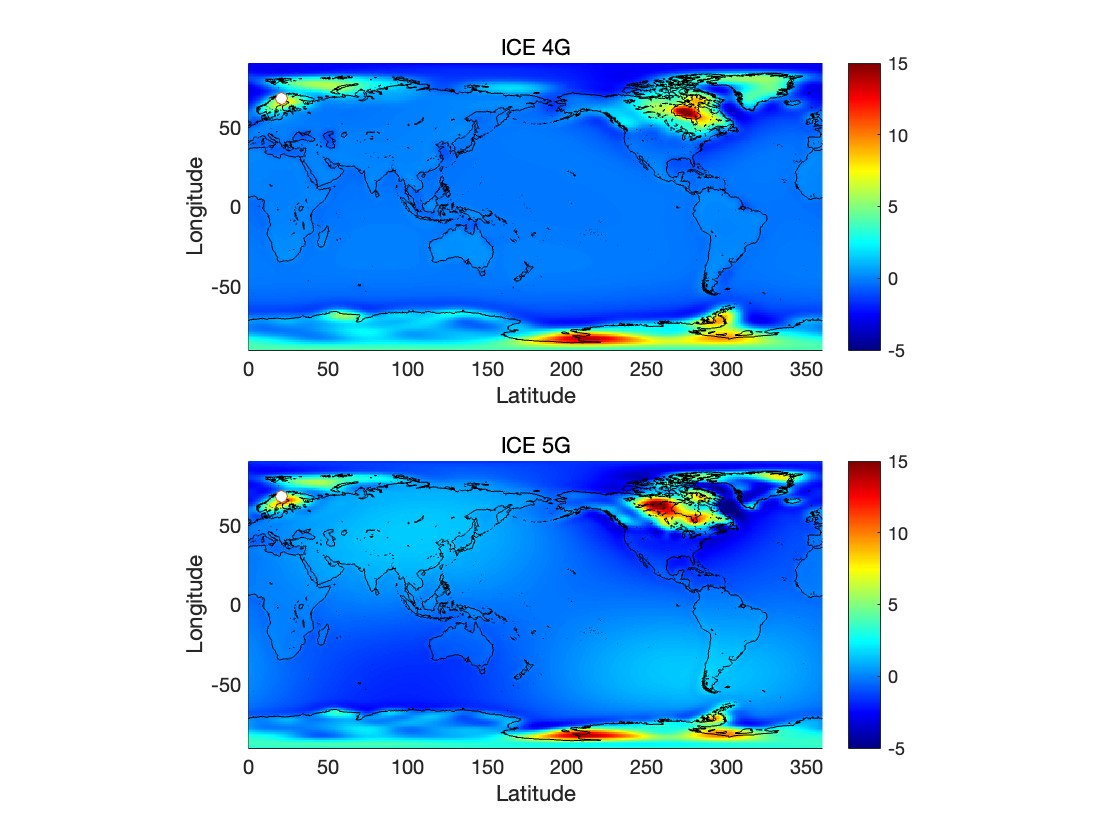
\includegraphics[width=11cm]{../result/re_figure/fig_kiru/1.jpg}
  \captionsetup{skip=0.2cm}
  \caption{GIA Model}
  \label{fig:GIA_global}
\end{figure}

At the same time, out group interpolate the vertical movements rates to the position of three stations, and the results are shown below:
\begin{figure}[H]
  \centering
  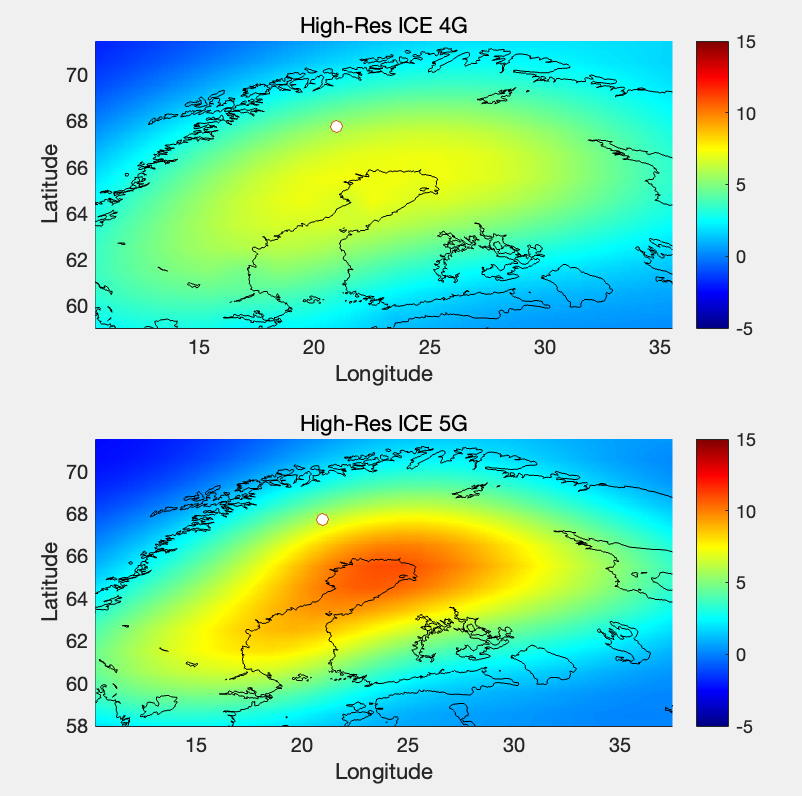
\includegraphics[width=9cm]{../result/ice/KIRU.png}
  \captionsetup{skip=0.2cm}
  \caption{GIA Model Interpolation at KIRU}
  \label{fig:GIA_KIRU}
\end{figure}
\begin{figure}[H]
  \centering
  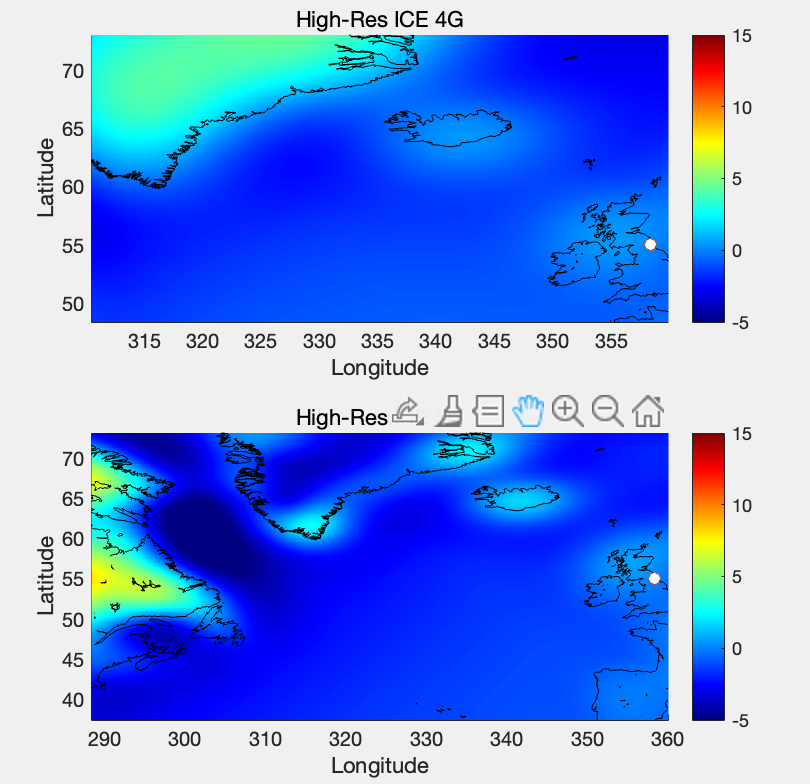
\includegraphics[width=9cm]{../result/ice/MORP.png}
  \captionsetup{skip=0.2cm}
  \caption{GIA Model Interpolation at MORP}
  \label{fig:GIA_MORP}
\end{figure}
\begin{figure}[H]
  \centering
  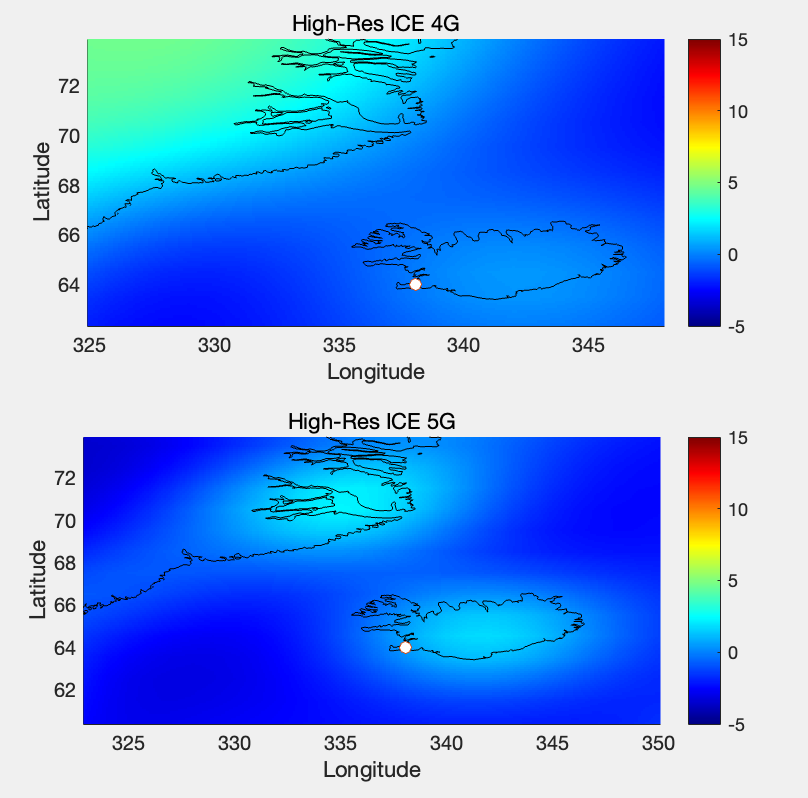
\includegraphics[width=9cm]{../result/ice/REYK.png}
  \captionsetup{skip=0.2cm}
  \caption{GIA Model Interpolation at REYK}
  \label{fig:GIA_REYK}
\end{figure}

The following table shows the specific values:
\vspace{5pt}
\begin{table}[htbp]
  \centering
  \caption{Vertical Movements Rates}
  \captionsetup{skip=0.2cm}
    \begin{tabular}{@{}cc@{\hspace{1.5cm}}cc@{}cc@{}}
      \midrule
    \large Station & \multicolumn{3}{c}{\large Vertical Movements Rates at IGS stations/(mm/y)} \\
    \midrule
          & \multicolumn{1}{c}{\large GNSS}& \large ICE-4G & \large ICE-5G \\ [4pt]
    \large KIRU  & \hspace{1.5cm} 6.8840 & 5.5568 & 6.1335 \\ [4pt]
    \large MORP  & \hspace{1.5cm} 0.4115 & 0.0140 & -0.0408 \\[4pt]
    \large REYK  & \hspace{1.5cm} 0.7212 & -0.0464 & 0.7236 \\
    \end{tabular}
  \label{tab:vert_vel}%
\end{table}%
\vspace{5pt}

So we can see that


\end{document}
